%\documentclass[12pt,letter,oneside]{article}

%\documentclass[12pt,onecolumn]{acmsiggraph}

\documentclass[12pt, letterpaper, onecolumn]{article}
\usepackage[top=1.0in, bottom=1.0in, left=1.0in, right=1.0in]{geometry} %onecolumn


\usepackage[dvips]{graphicx}
\usepackage{color}\pagecolor{white}
\usepackage{epsfig}
\usepackage{graphicx}
\usepackage{amsmath}
\usepackage{amsfonts}
\usepackage{latexsym}
\usepackage{bm}
%\usepackage{html,htmllist}


\graphicspath{{figures/}}
\usepackage{subfigure}

\usepackage{wrapfig}
\usepackage{parskip}

\def\R{\mathbb{R}}
\newenvironment{proof}{{\it Proof:\ } }{\hfill$\Box$ }
%\pagestyle{headings}

%\newcommand{\dspaceon}{\renewcommand{\baselinestretch}{1.3}\large\normalsize}
%\newcommand{\dspaceoff}{\renewcommand{\baselinestretch}{1}\large\normalsize}

%% editing comment

%\newcommand{\cmt}[1]{\textcolor{red}{\textbf {#1}}}
\newcommand{\cmt}[1]{}
\newcommand{\note}[1]{\cmt{Note: #1}}
\newcommand{\karen}[1]{\textcolor{blue}{{Karen: #1}}}
\newcommand{\sumit}[1]{\textcolor{red}{{Sumit: #1}}}
\newcommand{\newtext}[1]{#1}
%\newcommand{\newtext}[1]{\textcolor{blue}{#1}}
\newcommand{\eqnref}[1]{Equation~(\ref{eq:#1})}

%% ignore text
\long\def\ignorethis#1{}

%% abbreviations
\newcommand{\etal}{{\em{et~al.}\ }}
\newcommand{\eg}{e.g.\ }
\newcommand{\ie}{i.e.\ }

%% reference shortcuts
\newcommand{\figtodo}[1]{\framebox[0.8\columnwidth]{\rule{0pt}{1in}#1}}
\newcommand{\figref}[1]{Figure~\ref{fig:#1}}
%\renewcommand{\eqref}[1]{Equation~(\ref{eq:#1})}
\newcommand{\secref}[1]{Section~\ref{sec:#1}}

%% frequently used mathematical structures
\newcommand{\vc}[1]{\ensuremath{\mathbf{#1}}}
\newcommand{\pd}[2]{\ensuremath{\frac{\partial{#1}}{\partial{#2}}}}
\newcommand{\pdd}[3]{\ensuremath{\frac{\partial^2{#1}}{\partial{#2}\,\partial{#3}}}}


% math macros for phylter
\newcommand{\mTrans}{\ensuremath{\vc{T}}}
\newcommand{\vLinMom}{\ensuremath{\vc{P}}}
\newcommand{\vAngMom}{\ensuremath{\vc{L}}}
\newcommand{\vMomVar}{\ensuremath{\vc{u}}}
\newcommand{\vLine}{\ensuremath{\vc{l}}}
\newcommand{\vControlPoint}{\ensuremath{\vc{p}}}
\newcommand{\vControlKnot}{\ensuremath{\vc{u}}}

% math macros for style
\newcommand{\vStyle}{\ensuremath{\mathbf{\theta}}}
\newcommand{\sMusclePref}{\ensuremath{\alpha}}
\newcommand{\sKinetics}{\ensuremath{T}}
\newcommand{\sSpringCoef}{{\ensuremath{k_{s}}}}
\newcommand{\sDamperCoef}{{\ensuremath{k_{d}}}}
\newcommand{\sSpringCoefPos}{{\ensuremath{k_{s1}}}}
\newcommand{\sSpringCoefNeg}{{\ensuremath{k_{s2}}}}
\newcommand{\vLagrange}{\ensuremath{\vc{\lambda}}}
\newcommand{\sLagrange}{\ensuremath{\lambda}}
\newcommand{\sShoeRestLen}{\ensuremath{\bar{h}}}
\newcommand{\sShoeDist}{\ensuremath{h}}
\newcommand{\sShoeCoef}{{\ensuremath{k_{\mathit{shoe}}}}}
\newcommand{\vHandle}{\ensuremath{\vc{h}}}
\newcommand{\temp}{\ensuremath{\tau}}

%% math macros for multi-char
\newcommand{\vJointCoef}{{\ensuremath{\vc{h}_{q}}}}
\newcommand{\vTimeCoef}{\ensuremath{\vc{h}_t}}
\newcommand{\sTimeWarpFunc}{\ensuremath{F_t}}

%% math macros for phoward
%\newcommand{\vForce}{\ensuremath{\vc{f}}}
\newcommand{\sObjFunc}{\ensuremath{E}}
\newcommand{\vConeCoef}{\ensuremath{\vc{w}}}
\newcommand{\sConeCoef}{\ensuremath{w}}

%% frequently used symbols
\newcommand{\mTransChain}{\ensuremath{\vc{W}}}
\newcommand{\mRotateTrans}{\ensuremath{\vc{R}}}
\newcommand{\sJoint}{\ensuremath{q}}
\newcommand{\vJoint}{\ensuremath{\vc{q}}}
\newcommand{\mJoint}{\ensuremath{\vc{Q}}}
\newcommand{\mMass}{\ensuremath{\vc{M}}}
\newcommand{\mUnknown}{\ensuremath{\vc{X}}}
\newcommand{\sMass}{\ensuremath{{m}}}
\newcommand{\sInfMass}{\ensuremath{\mathbf{\mu}}}
\newcommand{\vGravity}{\ensuremath{\vc{g}}}
\newcommand{\vConstr}{\ensuremath{\vc{C}}}
\newcommand{\sConstr}{\ensuremath{C}}
\newcommand{\mGeometry}{\ensuremath{\vc{V}}}
\newcommand{\vCOM}{\ensuremath{\vc{c}}}
\newcommand{\sNumJoint}{\ensuremath{n_j}}
\newcommand{\sNumFrame}{\ensuremath{n_f}}
\newcommand{\sNumConstr}{\ensuremath{n_c}}
\newcommand{\sNumParticle}{\ensuremath{n_p}}
\newcommand{\vGlobalPoint}{\ensuremath{\vc{r}}}
\newcommand{\vLocalPoint}{\ensuremath{\vc{x}}}
\newcommand{\sGeneralForce}[1]{\ensuremath{Q_{#1}}}
\newcommand{\vForce}[1]{\ensuremath{\vc{f}_{#1}}}
\newcommand{\sWork}{\ensuremath{W}}
\newcommand{\vStateVar}{\ensuremath{\vc{y}}}
\newcommand{\vControlVar}{\ensuremath{\vc{u}}}
%\newcommand{\sObjFunc}{\ensuremath{F}}
\newcommand{\sCurve}{\ensuremath{S}}
\newcommand{\vCurve}{\ensuremath{\vc{S}}}
\newcommand{\argmax}{\operatornamewithlimits{argmax}}
\newcommand{\argmin}{\operatornamewithlimits{argmin}}


\newcommand{\tr}[1]{\ensuremath{\mathrm{tr}\left(#1\right)}}




%%%%%%%%%%%%%%%%%%%%%%%%%%%%%%%%%%%%%%%%%%%%%%%%%%%%%%%%%%%%%%%%%%%
%
% Here are a bunch of macros, mostly for math.
%
%%%%%%%%%%%%%%%%%%%%%%%%%%%%%%%%%%%%%%%%%%%%%%%%%%%%%%%%%%%%%%%%%%%

\renewcommand{\choose}[2]{\ensuremath{\left(\begin{array}{c} #1 \\ #2 \end{array} \right )}}

\newcommand{\gauss}[3]{\ensuremath{\mathcal{N}(#1 | #2 ; #3)}}

\newcommand{\pctab}{\hspace{0.2in}}
\newenvironment{pseudocode} {\begin{center} \begin{minipage}{\textwidth}
                             \normalsize \vspace{-2\baselineskip} \begin{tabbing}
                             \pctab \= \pctab \= \pctab \= \pctab \=
                             \pctab \= \pctab \= \pctab \= \pctab \= \\}
                            {\end{tabbing} \vspace{-2\baselineskip}
                             \end{minipage} \end{center}}
\newenvironment{items}      {\begin{list}{$\bullet$}
                              {\setlength{\partopsep}{\parskip}
                                \setlength{\parsep}{\parskip}
                                \setlength{\topsep}{0pt}
                                \setlength{\itemsep}{0pt}
                                \settowidth{\labelwidth}{$\bullet$}
                                \setlength{\labelsep}{1ex}
                                \setlength{\leftmargin}{\labelwidth}
                                \addtolength{\leftmargin}{\labelsep}
                                }
                              }
                            {\end{list}}
\newcommand{\newfun}[3]{\noindent\vspace{0pt}\fbox{\begin{minipage}{3.3truein}\vspace{#1}~ {#3}~\vspace{12pt}\end{minipage}}\vspace{#2}}



\newcommand{\key}{\textbf}
\newcommand{\fun}{\textsc}

\def\shortcite{\def\citename##1{}\@internalcite}


% Local Variables:
% TeX-master: "paper"
% End:


%
\def\sharedaffiliation{%
\end{tabular}
\begin{tabular}{c}}
%

\title{A Quick Tutorial on Multibody Dynamics}
\author{{C. Karen Liu} \\
{Sumit Jain} \\ \\ \\
{School of Interactive Computing}\\
{Georgia Institute of Technology} 
}

\begin{document}
\pagenumbering{roman}
%
\date{}
\maketitle

\newpage

\tableofcontents
\pagenumbering{arabic}
\newpage
%\section{Introduction}

This article attempts to answer the following questions.

\begin{itemize}
\item I know how to derive the equations of motion for one rigid body
  and I have seen people use the following equations for articulated
  rigid bodies, but I don't know how they are derived?
\begin{equation}
M(\vc{q}) \ddot{\vc{q}} + C(\vc{q}, \dot{\vc{q}})  = \vc{Q} \nonumber
\end{equation}

\item I have seen Lagrangian equation in the following form before, but I
  don't know how it is related to the equations of motion above.
\begin{equation}\label{eq:lagrangian_dyn}
    \frac{d}{dt} \left( \frac{\partial \sKinetics_i}{\partial
    \dot{\vJoint}} \right) - \frac{\partial \sKinetics_i}{\partial
    \vJoint} - \vc{Q} = 0 \nonumber
\end{equation}

\item I use generalized coordinates to compute the control forces, how do I convert them to Cartesian forces such that I can use simulators like ODE, PhysX, or Bullet which represent rigid bodies in the maximal coordinates?
\item I heard of Featherstone algorithm. What is it and how is it related to Lagrangian dynamics?
\end{itemize}

\section{Lagrangian Dynamics}
\label{sec:lagrangian}
Articulated human motions can be described by a set of dynamic
equations of motion of multibody systems. Since the direct
application of Newton's second law becomes difficult when a
complex human skeleton is considered, we use \emph{Lagrange's
equations} derived from \emph{D'Alembert's principle} to describe
the dynamic of the motions. The entire human skeleton is consist
of a collection of particles $\{\vGlobalPoint_1, \vGlobalPoint_2,
\ldots, \vGlobalPoint_{\sNumParticle}\}$.  Each particle,
$\vGlobalPoint_i$, is defined by Cartesian coordinates that
describe the translation with respective to the world coordinates.
We can represent $\vGlobalPoint_i$ by a set of \emph{generalized
coordinates} that indicate the joint configuration of the human
skeleton:

\begin{equation}\label{eq:general_coord}
    \vGlobalPoint_i = \vGlobalPoint_i(\sJoint_{1},
\sJoint_{2}, \ldots, \sJoint_{\sNumJoint}, t)
\end{equation}
where $t$ is the time and $\sJoint_j$ is a joint angle value in
the skeleton.

The virtual displacement $\delta \vGlobalPoint_i$ refers to an
infinitesimal change in the system coordinates such that the
constraint remains satisfied. In the context of human skeleton, the
system coordinates are the generalized coordinates $\sJoint_j$ and the
constraint manifold lies in the Cartesian space. The virtual
displacement $\delta \vGlobalPoint_i$ is a tangent vector to the
constraint manifold at a fixed time, written as

\begin{equation}\label{eq:virtual_displace}
    \delta \vGlobalPoint_i = \sum_j \frac{\partial \vGlobalPoint_i}{\partial
    \sJoint_j}\delta \sJoint_j
\end{equation}

We can write virtual work of force $\vForce{i}$ acting on particle
$\vGlobalPoint_i$ as
\begin{equation}\label{eq:virtual_work}
  \vForce{i} . \delta \vGlobalPoint_i = \vForce{i} . \sum_j \frac{\partial \vGlobalPoint_i}{\partial
    \sJoint_j}\delta \sJoint_j = \sum_j \sGeneralForce{j} \delta \sJoint_j
\end{equation}
where $\sGeneralForce{j} = \left ( \frac{\partial \vc{r}_i}{\partial q_j} \right )^T \vc{f}_i$ is defined as \emph{generalized force}
associated with coordinate $\sJoint_j$.

From D'Alembert's principle, we know that the sum of the differences
between the forces acting on a system and the inertia force of the
system along any virtual displacement consistent with the constraints
of the system, is zero. Therefore, the virtual work at $\vGlobalPoint_i$ can be written as
\begin{equation}\label{eq:inertial_work}
  \delta \sWork_i = \vForce{i} . \delta \vGlobalPoint_i = \sInfMass_i \ddot{\vGlobalPoint}_i \cdot
    \delta \vGlobalPoint_i = \sum_j \sInfMass_i \ddot{\vGlobalPoint}_i \cdot
    \frac{\partial \vGlobalPoint_i}{\partial \sJoint_j} \delta \sJoint_j
\end{equation}
where $\sInfMass_i$ is the infinitesimal mass associated with
$\vGlobalPoint_i$. The component of inertia force associated with
$\sJoint_j$ can be written as
\begin{equation}
\label{eq:inertia_force}
  \sInfMass_i \ddot{\vGlobalPoint}_i \cdot \frac{\partial \vGlobalPoint_i}{\partial \sJoint_j} =
  \frac{d}{dt} \left( \sInfMass_i \dot{\vGlobalPoint}_i \cdot \frac{\partial
  \vGlobalPoint_i}{\partial \sJoint_j} \right) - \sInfMass_i
\dot{\vGlobalPoint}_i \cdot \frac{d}{dt} \left( \frac{\partial
    \vGlobalPoint_i}{\partial \sJoint_j} \right) 
\end{equation}

Now let us consider the velocity of $\vGlobalPoint_i$ in terms of
joint velocity $\dot{\sJoint}_j$
\begin{equation}
\label{eq:velocity}
\dot{\vGlobalPoint}_i = \sum_j \frac{\partial
  \vGlobalPoint_i}{\partial \sJoint_j} \dot{\sJoint}_j
\end{equation}
from which we derive the following two identities:
\begin{eqnarray}
\frac{\partial \dot{\vGlobalPoint}_i}{\partial \dot{\sJoint}_j} &=&
\frac{\partial \vGlobalPoint_i}{\partial \sJoint_j}  \\
\frac{\partial \dot{\vGlobalPoint}_i}{\partial \sJoint_j} &=&
\sum_k \frac{\partial^2 \vGlobalPoint_i}{\partial \sJoint_j \partial
  \sJoint_k} \dot{\sJoint}_k = \frac{d}{dt} \frac{\partial \vGlobalPoint_i}{\partial \sJoint_j}
\end{eqnarray}

Using these two identities, we rewrite \eqnref{inertia_force} as
\begin{equation}
\label{eq:inertia_force2}
\sInfMass_i \ddot{\vGlobalPoint}_i \cdot \frac{\partial \vGlobalPoint_i}{\partial \sJoint_j}   = \frac{d}{dt} \left ( \frac{\partial}{\partial \dot{\sJoint}_j} \left( \frac{1}{2} \sInfMass_i \dot{\vGlobalPoint}_i^{T} \dot{\vGlobalPoint}_i\right) \right)
   - \frac{\partial}{\partial \sJoint_j} \left( \frac{1}{2} \sInfMass_i \dot{\vGlobalPoint}_i^{T} \dot{\vGlobalPoint}_i \right)
\end{equation}

We can denote the kinetic energy of $\vGlobalPoint_i$ as
\begin{equation}\label{eq:kinetic_energy}
    \sKinetics_i = \frac{1}{2} \sInfMass \dot{\vGlobalPoint}_i^{T}
    \dot{\vGlobalPoint}_i,
\end{equation}
and rewrite \eqnref{inertia_force2} as
\begin{equation}\label{eq:inertia_kinetic}
    \sInfMass_i \ddot{\vGlobalPoint}_i \cdot \frac{\partial \vGlobalPoint_i}{\partial
    \sJoint_j} = \frac{d}{dt} \left( \frac{\partial \sKinetics_i}{\partial
    \dot{\sJoint}_j}\right) - \frac{\partial \sKinetics_i}{\partial \sJoint_j}
\end{equation}

Combining the definition of generalized force (\eqnref{virtual_work}), D'Alembert's principle (\eqnref{inertial_work}), and the generalized inertia force (\eqnref{inertia_kinetic}), we arrive at the following equation:
\begin{equation}\label{eq:dynamic_equil}
    \left ( \frac{d}{dt} \left( \frac{\partial \sKinetics_i}{\partial \dot{\sJoint}_j} \right) - \frac{\partial \sKinetics_i}{\partial
    \sJoint_j}\right ) \delta \sJoint_j = \sGeneralForce{j} \delta
    \sJoint_j
\end{equation}

If the set of generalized coordinates $\sJoint_j$ is linearly
independent, \eqnref{dynamic_equil} leads to
\emph{Lagrangian equation}:
\begin{equation}\label{eq:lagrangian_dyn2}
    \frac{d}{dt} \left( \frac{\partial \sKinetics_i}{\partial
    \dot{\sJoint}_j} \right) - \frac{\partial \sKinetics_i}{\partial
    \sJoint_j} - \sGeneralForce{j} = 0
\end{equation}

\paragraph{Equations of Motion in Vector Form.} \eqnref{lagrangian_dyn2} is the equation of motion for one generalized coordinate in a
multibody system. We can combine $\sNumJoint$  scalar equations into
the familiar vector form
\begin{equation}\label{eq:lagrangian_vector}
M(\vc{q}) \ddot{\vc{q}} + C(\vc{q}, \dot{\vc{q}}) = \vc{Q} 
\end{equation}
where $M(\vc{q})$ is the mass matrix, $C(\vc{q}, \dot{\vc{q}})$ is the
Coriolis and centrifugal term of the equation of motion, and $\vc{Q}$
is the vector of generalized forces for all the degrees of freedom
(DOFs) in the system. $M$ only depends on $\vc{q}$ and $C$ depends
quadratically on $\dot{\vc{q}}$.

How do we derive $M$ and $C$ from \eqnref{lagrangian_dyn2}?
Let us go back to the velocity of one particle $\vGlobalPoint_i$:
\begin{equation}
\dot{\vGlobalPoint}_i = \sum_j \frac{\partial
  \vGlobalPoint_i}{\partial \sJoint_j} \dot{\sJoint}_j = J_i(\vc{q}) \dot{\vc{q}}
\end{equation}
where $J_i$ denotes the Jacobian of $\vGlobalPoint_i$. By summing up
all the particles in the system, the kinetic
energy of the system can then be expressed as
\begin{equation}
\label{eq:kinetic_vector}
T = \sum_i T_i = \sum_i \frac{1}{2}  \sInfMass \dot{\vGlobalPoint}_i^{T}
    \dot{\vGlobalPoint}_i = \sum_i \frac{1}{2}  \sInfMass (J_i
    \dot{\vc{q}})^T(J_i \dot{\vc{q}}) = \frac{1}{2} \dot{\vc{q}}^T
    (\sum_i \sInfMass J_i^TJ_i) \dot{\vc{q}} = \frac{1}{2}
    \dot{\vc{q}}^T M(\vc{q}) \dot{\vc{q}}
\end{equation}
where we define the mass matrix, $M(\vc{q}) = \sum_i \sInfMass
J_i^TJ_i$, and will shortly show it is indeed the mass matrix in
\eqnref{lagrangian_vector}.

From \eqnref{kinetic_vector}, we can derive the derivative
terms to construct the Lagrange's equation (\eqnref{lagrangian_dyn2}).
\begin{equation}
\frac{d}{dt}\frac{\partial T}{\partial \dot{\vc{q}}} - \frac{\partial
  T}{\partial \vc{q}} = M\ddot{\vc{q}} + \dot{M} \dot{\vc{q}} - \frac{1}{2}\dot{\vc{q}}^T \left ( \frac{\partial M}{\partial \vc{q}} \right )^T \dot{\vc{q}} \equiv M
\ddot{\vc{q}} + C(\vc{q}, \dot{\vc{q}})
\end{equation}
where $C$ is the Coriolis and centrifugal term in \eqnref{lagrangian_vector} and is defined as $C = \dot{M}
\dot{\vc{q}} - \frac{1}{2}\left( \frac{\partial M}{\partial  \vc{q}} \dot{\vc{q}} \right)^T \dot{\vc{q}}$. 

\paragraph{Note.} In the second term of $C$, we introduce tensor notation $\frac{\partial M}{\partial \vc{q}}$, which implies that the $j^{th}$ element of the tensor $\frac{\partial M}{\partial \vc{q}}$ is the matrix $\frac{\partial M}{\partial {q}_j}$. Note that, in general, the quantity with notation $\frac{\partial M}{\partial \vc{q}} \dot{\vc{q}}$ is \textbf{\emph{not}} equal to $\dot{M}$. This is because, the $j^{th}$ column of the matrix $\frac{\partial M}{\partial \vc{q}} \dot{\vc{q}}$ is the vector $\frac{\partial M}{\partial q_j} \dot{\vc{q}}$ or $\sum_k \frac{\partial (M)_k}{\partial q_j} \dot{{q}_k}$, where the notation $(A)_j$ denotes the $j^{th}$ column of the matrix $A$. In contrast, the $j^{th}$ column of the matrix $\dot{M}$ is $\sum_k \frac{\partial (M)_j}{\partial q_k} \dot{{q}_k}$.
\sumit{Not sure that they are equal ?}

Once we know how to compute the mass matrix, Coriolis and centrifugal
term, and generalized forces, we can compute the acceleration in
generalized coordinates, $\ddot{\vc{q}}$, for forward
simulation. Conversely, if we are given $\ddot{\vc{q}}$ from a motion
sequence, we can use these equations of motion to derive generalized
forces for inverse dynamics. 

The above formulation is convenient for a system consisting of finite number of mass points. However, for a dynamic system that consists of rigid bodies, there are infinitely many points contained in each rigid body making the above formulation intractable. The rigid body relation between the infinitely many points in a rigid body can be exploited to make the equations compact. In the following sections, we derive the equations of motions for a rigid body followed by the equations for an articulated multibody system.

\section{Rigid Body Dynamics: Newton-Euler equations}
We describe the familiar Newton-Euler equations of rigid body dynamics. We start writing down the
momenta of the rigid body whose mass, position of the center
of mass (COM), orientation,
linear velocity of the COM, and angular velocity are $m$, $\vc{x}$, $R$,
$\vc{v}$, and $\bm{\omega}$ respectively (same as defined in Witkin and
Baraff's course notes). The linear momentum \vc{p} is computed as:
\begin{eqnarray}
\vc{p} &=& \sum_i \vc{p}_i = \sum_i \sInfMass \dot{\vGlobalPoint}_i = \sum_i  \sInfMass (\vc{v} + \bm{\omega}
    \times \vc{r}_i') \nonumber \\
 &=& m \vc{v}
\end{eqnarray}
where $\vc{r}_i' = \vc{r}_i - \vc{x}$. Because $\sum_i \sInfMass
\vc{r}_i' = \vc{0}$ (property of the COM), the second term vanishes. The angular momentum \vc{L} about the COM is computed as:
\begin{eqnarray}
\nonumber
\vc{L} & = & \sum_i \vc{L}_i  = \sum_i \vc{r}_i' \times \vc{p}_i\\
\nonumber
& = & \sum_i \sInfMass \vc{r}_i' \times (\vc{v} + \bm{\omega} \times \vc{r}_i')\\
&= & \vc{0} + \sum_i \sInfMass [\vc{r}_i'][\bm{\omega}]\vc{r}_i' = \left ( \sum_i -\sInfMass [\vc{r}_i'][\vc{r}_i'] \right )\bm{\omega}
\end{eqnarray}
The notation $[\vc{a}] \vc{b}$ denotes the cross product $\vc{a}\times \vc{b}$ with $[\vc{a}]$ as the skew-symmetric matrix corresponding to the vector $\vc{a}$. Therefore the following identities hold: $[\vc{a}]\vc{b} = -[\vc{b}]\vc{a}$ and $[\vc{a}]^T = -[\vc{a}]$.

Now recall the inertia tensor about the COM defined in Witkin and
Baraff's course notes: $I_c = \sum_i \sInfMass ((\vc{r}_i'^T
\vc{r}_i')\vc{I}_3 - \vc{r}_i' \vc{r}_i'^T)$, where $\vc{I}_3$ is the $3\times 3$
identity matrix. We can easily show that
$I_c = \sum_i -\sInfMass [\vc{r}_i'][\vc{r}_i']$ by verifying the
identity $-[\vc{a}][\vc{a}] = (\vc{a}^T\vc{a}) \vc{I}_3  -
\vc{a}\vc{a}^T$. As a result, we write the angular momentum of a rigid body as:
\begin{equation}
\vc{L} = I_c \bm{\omega}
\end{equation}
Note that the inertia tensor can be written as $I_c = RI_0R^T$, where $R$ is the rotation matrix corresponding to the orientation of the body and $I_0$ is the constant inertia tensor defined at zero rotation. The angular velocity in the skew-symmetric form is related to the rotation matrix $R$ as $[\bm{\omega}] = \dot{R}R^T$. Also $[\bm{\omega}]^T = -[\bm{\omega}]$.

Now, the dynamics of a rigid body can be written as $\vc{f} = \dot{\vc{p}} \mbox{,\ } \bm{\tau} = \dot{\vc{L}}$. The equations corresponding to the linear force can be evaluated as:
\begin{eqnarray}
\label{eq:force}
\vc{f} & = & \dot{\vc{p}} = m \dot{\vc{v}}
\end{eqnarray}
The equations corresponding to the torque can be evaluated as:
\begin{eqnarray}
\label{eq:torque}
\nonumber
\bm{\tau} & = & \dot{\vc{L}} = \dot{(I_c \bm{\omega})} \\
\nonumber
& = & I_c\dot{\bm{\omega}} + \dot{(RI_0 R^T)}\bm{\omega} = I_c\dot{\bm{\omega}} + \dot{R}I_0 R^T\bm{\omega} + R I_0 \dot{R}^T\bm{\omega}\\
\nonumber
& = & I_c\dot{\bm{\omega}} + \dot{R}R^T I_c \bm{\omega} + I_c (\dot{R}R^T)^T\bm{\omega} \\
& = & I_c\dot{\bm{\omega}} + [\bm{\omega}]I_c \bm{\omega} - I_c[\bm{\omega}]\bm{\omega} = I_c\dot{\bm{\omega}} + \bm{\omega} \times I_c \bm{\omega}
\end{eqnarray}

Combining \eqnref{force} and \eqnref{torque}, we get:
\begin{equation}
\label{eq:newtoneuler}
\left(
\begin{array}{cc}
m\vc{I}_3 & \vc{0} \\
\vc{0} & I_c 
\end{array}
\right)
\left(
\begin{array}{c}
\dot{\vc{v}} \\
\dot{\bm{\omega}} 
\end{array}
\right) +
\left(
\begin{array}{c}
\vc{0}  \\
\bm{\omega} \times I_c \bm{\omega} 
\end{array}
\right) = 
\left(
\begin{array}{c}
\vc{f} \\
\bm{\tau} 
\end{array}
\right)
\end{equation}

\section{Rigid Body Dynamics: Generalized coordinates}
\label{sec:rigidbodydyngen}
The Newton-Euler equations are defined in terms of velocities instead of position and orientation. We now derive the equations in generalized coordinates \vc{q} that define the position and orientation. The first three coordinates are the same as the position of COM. The next three represent the rotation of the rigid body such as an exponential map or three Euler angles (or four coordinates can be used for a quaternion).

We first start by computing the kinetic energy of the rigid body:
\begin{eqnarray}
\label{eq:rigid_kinetic}
T &=& \sum_i T_i = \sum_i \frac{1}{2}  \sInfMass \dot{\vGlobalPoint}_i^{T}
    \dot{\vGlobalPoint}_i = \sum_i \frac{1}{2}  \sInfMass (\vc{v} + \bm{\omega}
    \times \vc{r}_i')^T (\vc{v} + \boldsymbol{\bm{\omega}}
    \times \vc{r}_i') \nonumber \\
 &=& \sum_i \frac{1}{2}  \sInfMass (\vc{v}^T\vc{v} +
    \vc{v}^T [\bm{\omega}] \vc{r}_i' + \vc{r}_i'^T [\bm{\omega}]^T \vc{v} +
    \vc{r}_i'^T [\bm{\omega}]^T [\bm{\omega}] \vc{r}_i')
\end{eqnarray}
Because $\sum_i \sInfMass
\vc{r}_i' = \vc{0}$, the second term and the third term in \eqnref{rigid_kinetic} vanish. Using the identity $[\bm{\omega}]\vc{r}_i' =
-[\vc{r}_i']\bm{\omega}$, we can rewrite \eqnref{rigid_kinetic}
as:
\begin{eqnarray}
\nonumber
T & = & \frac{1}{2} m \vc{v}^T\vc{v} + \frac{1}{2} \bm{\omega}^T \left ( \sum_i -\sInfMass
 [\vc{r}_i'][\vc{r}_i'] \right ) \bm{\omega}\\
 & = & \frac{1}{2} m \vc{v}^T\vc{v} + \frac{1}{2} \bm{\omega}^T I_c \bm{\omega}
\end{eqnarray}
The kinetic energy of a rigid body can be written in its vector form:
\begin{eqnarray}
\label{eq:kinetic_vec}
T &=& \frac{1}{2} (\vc{v}^T \;\; \bm{\omega}^T)
\left(
\begin{array}{cc}
m\vc{I}_3 & \vc{0} \\
\vc{0} & I_c
\end{array}
\right)
\left(
\begin{array}{c}
\vc{v} \\
\bm{\omega} 
\end{array}
\right)
 \equiv \frac{1}{2}\vc{V}^T M_c \vc{V}
\end{eqnarray}
where $\vc{V} = (\vc{v}^T,\bm{\omega}^T)^T$, $M_c = \mbox{blockdiag}(m\vc{I}_3,I_c)$. We now relate the velocities in the Cartesian space $\vc{V}$ to the generalized velocities $\dot{\vc{q}}$. Let $\vc{x}(\vc{q})$ and $R(\vc{q})$ represent the position of the COM and the rotation matrix of the rigid body. The linear velocity of the COM is computed as:
\begin{eqnarray}
\label{eq:vellin}
\vc{v} = \dot{\vc{x}}(\vc{q}) = \frac{\partial \vc{x}}{\partial \vc{q}} \dot{\vc{q}} \equiv J_v \dot{\vc{q}}
\end{eqnarray}
The angular velocity is computed as:
\begin{eqnarray}
\nonumber
[\bm{\omega}] & = & \dot{R}(\vc{q})R^T(\vc{q}) \\
\label{eq:Jaccolj}
& = & \sum_j \frac{\partial R}{\partial q_j}R^T \dot{q}_j \equiv \sum_j [\vc{j}_{j}] \dot{q}_j
\end{eqnarray}
$\frac{\partial R}{\partial q_j}R^T$ is always a skew-symmetric matrix that we represent as $[\vc{j}_{j}]$ (skew-symmetric form of the vector $\vc{j}_j$). $\bm{\omega}$ can be now be represented in the vector form as:
\begin{equation}
\label{eq:velang}
\bm{\omega} = J_{\omega} \dot{\vc{q}}
\end{equation}
where $\vc{j}_{j}$ is the $j^{th}$ column of the matrix $J_{\omega}$.

Using \eqnref{vellin} and \eqnref{velang}, we can write:
\begin{equation}
\label{eq:velcartall}
\vc{V} = \left(
\begin{array}{c}
J_v \\
J_{\omega}
\end{array}
\right) \dot{\vc{q}} \equiv J(\vc{q})\dot{\vc{q}}
\end{equation}
Substituting the above in \eqnref{kinetic_vec}, we get:
\begin{equation}
T = \frac{1}{2}\dot{\vc{q}}^T J^T M_c J \dot{\vc{q}}
\end{equation}

Using the recipe of Lagrangian dynamics in \eqnref{lagrangian_dyn2}, we first compute $\frac{\partial T}{\partial \dot{q}_j}$ as:
\begin{eqnarray}
\nonumber
\frac{\partial T}{\partial \dot{q}_j} & = & \frac{1}{2}\dot{\vc{q}}^T J^T M_c (J)_j + \frac{1}{2} (J)_j^T M_c J \dot{\vc{q}}\\
 & = & (J)_j^T M_c J \dot{\vc{q}}
\end{eqnarray}
where the notation $(A)_j$ denotes the $j^{th}$ column of the matrix A. The term $\frac{d}{dt} \left( \frac{\partial T}{\partial \dot{q}_j} \right )$ is computed as:
\begin{eqnarray}
\label{eq:lagterm1}
\frac{d}{dt} \left ( \frac{\partial T}{\partial \dot{q}_j} \right ) & = & (J)_j^T M_c J \ddot{\vc{q}} + (J)_j^T M_c \dot{J} \dot{\vc{q}} + (J)_j^T \dot{M}_c J \dot{\vc{q}} + \dot{(J)}_j^T M_c J \dot{\vc{q}}
\end{eqnarray}
Now we evaluate the term $\frac{\partial T}{\partial q_j}$:
\begin{eqnarray}
\nonumber
\frac{\partial T}{\partial q_j} & = & \frac{1}{2}\dot{\vc{q}}^T J^T M_c \frac{\partial J}{\partial q_j} \dot{\vc{q}} + \frac{1}{2}\dot{\vc{q}}^T J^T \frac{\partial M_c}{\partial q_j} J \dot{\vc{q}} + \frac{1}{2}\dot{\vc{q}}^T \frac{\partial J^T}{\partial q_j} M_c J \dot{\vc{q}}\\
\label{eq:lagterm2}
& = & \dot{\vc{q}}^T \frac{\partial J^T}{\partial q_j} M_c J \dot{\vc{q}} + \frac{1}{2}\dot{\vc{q}}^T J^T \frac{\partial M_c}{\partial q_j} J \dot{\vc{q}}
\end{eqnarray}
Using the above equations, we write:
\begin{eqnarray}
\label{eq:lageqn_j}
\nonumber
\frac{d}{dt} \left ( \frac{\partial T}{\partial \dot{q}_j} \right ) - \frac{\partial T}{\partial q_j} & = & (J)_j^T M_c J \ddot{\vc{q}} + (J)_j^T M_c \dot{J} \dot{\vc{q}} + (J)_j^T \dot{M}_c J \dot{\vc{q}} - \frac{1}{2}\dot{\vc{q}}^T J^T \frac{\partial M_c}{\partial q_j} J \dot{\vc{q}} \\ & & + \left ( \dot{(J)}_j^T M_c J \dot{\vc{q}}  - \left( \frac{\partial J}{\partial q_j} \dot{\vc{q}}\right)^T M_c J \dot{\vc{q}} \right )
\end{eqnarray}

The second term in the above equation involves the computation of $\dot{J}$ that can be computed as $\sum_k \frac{\partial J}{\partial q_k} \dot{q}_k$. We now simplify the third, fourth and the fifth terms one by one. Let us start with the third term:
\begin{eqnarray}
\label{eq:term3}
\nonumber
(J)_j^T \dot{M}_c J \dot{\vc{q}} & = & (J_w)_j^T \dot{I}_c J_w \dot{\vc{q}} \mbox{\ \ (The linear term in $M_c$ is constant: see \eqnref{kinetic_vec})}\\
\nonumber
& = & \vc{j}_j^T\dot{(RI_0 R^T)}\bm{\omega} \mbox{\ \ ($\vc{j}_j$ represents the $j^{th}$ column of $J_w$: see \eqnref{Jaccolj})} \\
\mbox{term 3} & = & \vc{j}_j^T[\bm{\omega}]I_c \bm{\omega}  \mbox{\ \ (From \eqnref{torque})}
\end{eqnarray}
The fourth term in \eqnref{lageqn_j} can be simplified as:
\begin{eqnarray}
\label{eq:term4}
\nonumber
\frac{1}{2}\dot{\vc{q}}^T J^T \frac{\partial M_c}{\partial q_j} J \dot{\vc{q}} & = & \frac{1}{2} (J_w \dot{\vc{q}})^T \frac{\partial I_c}{\partial q_j} J_w \dot{\vc{q}}\\
\nonumber
& = & \frac{1}{2} \bm{\omega}^T \left ( \frac{\partial R}{\partial q_j}I_0R^T + RI_0\frac{\partial R^T}{\partial q_j} \right )  \bm{\omega} = \bm{\omega}^T \left ( \frac{\partial R}{\partial q_j}I_0R^T \right ) \bm{\omega} \\
\nonumber
& = & \bm{\omega}^T \left ( \frac{\partial R}{\partial q_j}R^T I_c \right ) \bm{\omega}\\
\nonumber
 & = & \bm{\omega}^T [\vc{j}_j] I_c \bm{\omega} \mbox{\ \ (From \eqnref{Jaccolj})}\\
\mbox{term 4}  & = & - \vc{j}_j^T[\bm{\omega}]I_c \bm{\omega} \mbox{\ \ (Using the identity $\vc{a}.(\vc{b}\times\vc{c}) = -\vc{b}.(\vc{a}\times\vc{c}))$}
\end{eqnarray}
For simplifying the fifth term in \eqnref{lageqn_j}, we explicitly express it using the linear and angular components:
\begin{eqnarray}
\label{eq:term5}
\left (
\begin{array}{cc}
\dot{(J_v)_j}^T & \dot{(J_\omega)_j}^T
\end{array} 
\right )
\left(
\begin{array}{cc}
m\vc{I}_3 & \vc{0} \\
\vc{0} & I_c
\end{array}
\right)
\left (
\begin{array}{cc}
J_v \dot{\vc{q}} \\
J_\omega \dot{\vc{q}}
\end{array} 
\right )
-
\left (
\begin{array}{cc}
\left(\frac{\partial J_v}{\partial q_j}\dot{\vc{q}}\right)^T & \left(\frac{\partial J_\omega}{\partial q_j}\dot{\vc{q}}\right)^T
\end{array} 
\right )
\left(
\begin{array}{cc}
m\vc{I}_3 & \vc{0} \\
\vc{0} & I_c
\end{array}
\right)
\left (
\begin{array}{cc}
J_v \dot{\vc{q}} \\
J_\omega \dot{\vc{q}}
\end{array} 
\right )
\end{eqnarray}
The linear term can be extracted and simplified as:
\begin{eqnarray}
\label{eq:term5_lin}
\nonumber
m\left( \dot{(J_v)_j}  - \left(\frac{\partial J_v}{\partial q_j}\dot{\vc{q}}\right) \right )^T J_v \dot{\vc{q}} & = & m\left( \sum_k \frac{\partial (J_v)_j}{\partial q_k}\dot{q}_k -  \sum_k \frac{\partial (J_v)_k}{\partial q_j} \dot{q}_k \right )^T J_v \dot{\vc{q}}\\
\nonumber
& = & m\left( \sum_k \frac{\partial^2 \vc{x}}{\partial q_j \partial q_k}\dot{q}_k -  \sum_k \frac{\partial^2 \vc{x}}{\partial q_k \partial q_j} \dot{q}_k \right )^T J_v \dot{\vc{q}} \\
\mbox{term 5 (linear)} & = & 0
\end{eqnarray}
The above derivation uses the property of the Jacobian of the linear velocity  $(J_v)_j = \frac{\partial \vc{x}}{\partial q_j}$ $\forall j$ (See \eqnref{vellin}).

We now extract and simplify the angular term in \eqnref{term5} as:
\begin{eqnarray}
\label{eq:term5_ang}
\nonumber
\left( \dot{(J_\omega)_j}  - \left(\frac{\partial J_\omega}{\partial q_j}\dot{\vc{q}}\right) \right )^T I_c J_\omega \dot{\vc{q}} & = & \left( \sum_k \frac{\partial \vc{j}_j}{\partial q_k}\dot{q}_k -  \sum_k \frac{\partial \vc{j}_k}{\partial q_j} \dot{q}_k \right )^T I_c \bm{\omega}\\
& = & \left( \sum_k \left ( \frac{\partial \vc{j}_j}{\partial q_k}  -  \frac{\partial \vc{j}_k}{\partial q_j}\right ) \dot{q}_k \right )^T I_c \bm{\omega} \equiv \left ( \sum_k \vc{z}_{jk} \dot{q}_k \right )^T I_c\bm{\omega} 
\end{eqnarray}
Now let us evaluate the term denoted by $\vc{z}_{jk}$. Consider the skew symmetric form:
\begin{eqnarray}
\nonumber
[\vc{z}_{jk}] & = & \left [ \frac{\partial \vc{j}_j}{\partial q_k}  -  \frac{\partial \vc{j}_k}{\partial q_j} \right ] = \frac{\partial [\vc{j}_j]}{\partial q_k}  -  \frac{\partial [\vc{j}_k]}{\partial q_j} \mbox{\ \ (Using linearity of the skew symmetric matrix)}\\
\nonumber
& = & \left ( \frac{\partial^2 R}{\partial q_j \partial q_k} + \frac{\partial R}{\partial q_j} \frac{\partial R^T}{\partial q_k} \right ) - \left ( \frac{\partial^2 R}{\partial q_k \partial q_j} + \frac{\partial R}{\partial q_k} \frac{\partial R^T}{\partial q_j} \right ) \mbox{\ \ (From \eqnref{Jaccolj})}\\
\nonumber
& = & \frac{\partial R}{\partial q_j}R^T \left( \frac{\partial R}{\partial q_k}R^T\right)^T - \frac{\partial R}{\partial q_k}R^T \left( \frac{\partial R}{\partial q_j}R^T\right)^T\\
\nonumber
& = & -[\vc{j}_j][\vc{j}_k] + [\vc{j}_k][\vc{j}_j] \mbox{\ \ (Using the identity $[\vc{a}]^T = -[\vc{a}]$)}\\
\nonumber
& = & [\vc{j}_k\times \vc{j}_j] \mbox{\ \ (Using the identity $[\vc{u}\times \vc{v}] = [\vc{u}][\vc{v}] - [\vc{v}][\vc{u}]$)}\\
\Rightarrow \vc{z}_{jk} & = & \vc{j}_k\times \vc{j}_j = [\vc{j}_k] \vc{j}_j
\end{eqnarray}

Substituting the above in \eqnref{term5_ang}, we get:
\begin{eqnarray}
\label{eq:term5_ang_final}
\nonumber
\left ( \sum_k \vc{z}_{jk} \dot{q}_k \right )^T I_c\bm{\omega}  & = & \left ( \sum_k [\vc{j}_k] \vc{j}_j \dot{q}_k \right )^T I_c\bm{\omega} \\
\nonumber
& = & \left ( \bigg ( \sum_k [\vc{j}_k]\dot{q}_k \bigg ) \vc{j}_j \right )^T I_c\bm{\omega}\\
\nonumber
& = & \left ( \bigg [ \sum_k \vc{j}_k \dot{q}_k \bigg ] \vc{j}_j \right )^T I_c\bm{\omega} \\
\nonumber
& = & \left ( [ J_\omega \dot{\vc{q}} ] \vc{j}_j \right )^T I_c\bm{\omega} = ([\bm{\omega}]\vc{j}_j)^TI_c\bm{\omega}\\
\mbox{term 5 (angular)} & = & -\vc{j}_j^T [\bm{\omega}] I_c\bm{\omega}
\end{eqnarray} 

Finally, we substitute the terms computed in \eqnref{term3}, \eqnref{term4}, \eqnref{term5_lin} and \eqnref{term5_ang_final} into \eqnref{lageqn_j} and rewrite it as:
\begin{eqnarray}
\label{eq:lageqn_j_final}
\nonumber
\frac{d}{dt} \left ( \frac{\partial T}{\partial \dot{q}_j} \right ) - \frac{\partial T}{\partial q_j} & = & (J)_j^T M_c J \ddot{\vc{q}} + (J)_j^T M_c \dot{J} \dot{\vc{q}} + \vc{j}_j^T[\bm{\omega}]I_c \bm{\omega}\\
\nonumber
& = & \left( (J)_j^T M_c J \right )\ddot{\vc{q}} + \left( (J)_j^T M_c \dot{J} + (J)_j^T [\tilde{\bm{\omega}}]M_c J \right )\dot{\vc{q}}\\
\mbox{where } [\tilde{\bm{\omega}}] & = &
\left ( 
\begin{array}{cc}
\vc{0} & \vc{0} \\
\vc{0} & [J_\omega \dot{\vc{q}}]
\end{array}
\right )
\end{eqnarray}

Writing the equations for all the $q_j$ in the vector form, we get:
\begin{eqnarray}
\label{eq:dyngen_vec}
\frac{d}{dt} \left ( \frac{\partial T}{\partial \dot{\vc{q}}} \right ) - \frac{\partial T}{\partial \vc{q}} & = & \left( J^T M_c J \right )\ddot{\vc{q}} + \left( J^T M_c \dot{J} + J^T [\tilde{\bm{\omega}}]M_c J \right )\dot{\vc{q}}
\end{eqnarray}


\subsection{Derivation using Newton-Euler equations}
We can alternatively derive the result in \eqnref{dyngen_vec} from the Newton-Euler equations in \eqnref{newtoneuler}. Using \eqnref{velcartall}, we substitute the Cartesian velocities $\vc{v},\bm{\omega}$ in terms of the generalized velocities $\dot{\vc{q}}$ into \eqnref{newtoneuler} and get:
\begin{eqnarray}
\nonumber
M_c (\dot{J\dot{\vc{q}}}) + 
\left ( 
\begin{array}{c}
\vc{0} \\
(J_w \dot{\vc{q}}) \times I_c J_w \dot{\vc{q}}
\end{array}
\right )
& = &
\left ( 
\begin{array}{c}
\vc{f} \\
\bm{\tau}
\end{array}
\right )\\
\Rightarrow 
M_c J \ddot{\vc{q}} + M_c \dot{J} \dot{\vc{q}} + [\tilde{\bm{\omega}}]M_c J \dot{\vc{q}} & = & 
\left ( 
\begin{array}{c}
\vc{f} \\
\bm{\tau}
\end{array}
\right )
\end{eqnarray}

From the principle of virtual work in \eqnref{virtual_work}, we convert the Cartesian-space forces to the Generalized space by pre-multiplying the above equation with the transpose of the Jacobian $J$:
\begin{eqnarray}
\label{eq:dyngen_vec2}
\left (J^T M_c J \right ) \ddot{\vc{q}} + \left (J^T M_c \dot{J} + J^T [\tilde{\bm{\omega}}]M_c J \right ) \dot{\vc{q}} & = & J_v^T \vc{f} + J_\omega^T \bm{\tau}
\end{eqnarray}

The LHS of \eqnref{dyngen_vec2} is identical to the RHS of \eqnref{dyngen_vec} and they are of the form $M(\vc{q})\ddot{\vc{q}} + C(\vc{q},\dot{\vc{q}}) = \vc{Q}$, where the Mass matrix, the Coriolis matrix and the generalized forces are defined as:
\begin{eqnarray}
\label{eq:summary_dynamics}
\nonumber
M(\vc{q}) & = & J^T M_c J\\
\nonumber
C(\vc{q},\dot{\vc{q}}) & = & (J^T M_c \dot{J} + J^T [\tilde{\bm{\omega}}]M_c J)\dot{\vc{q}}\\
\vc{Q} & = & J_v^T \vc{f} + J_\omega^T \bm{\tau}
\end{eqnarray}

\section{Articulated Rigid Body Dynamics}
We now derive the equations of motion for an articulated rigid body structure. We follow the derivation of rigid body dynamics in generalized coordinates from \secref{rigidbodydyngen}.

An articulated rigid body system is represented as a set of rigid bodies connected through joints in a tree structure. Every rigid link has exactly one \emph{parent} joint. The joint corresponding to the root of the tree is special since it does not link the root to any other rigid link. The generalized coordinates are the six DOFs of the root link of the tree (that may represent the global translation and rotation), and the joint angles corresponding to the admissible joint rotations for all the other joints. 

\subsection{Definitions}
The state of an articulated rigid body
system can be expressed as $(\vc{x}_k, R_k, \vc{v}_k,
\boldsymbol{\bm{\omega}}_k)$, where $k = 1, \cdots, m$ and $m$ is the number of rigid links. Here $\vc{x}_k$ and
$R_k$ are the position and orientation of the rigid link $k$, and $(\vc{v}_k,
{\bm{\omega}}_k)$ are the linear and angular velocity of the
rigid link $k$ viewed in the world frame. Similarly, we define the
Cartesian force and torque applied on rigid link $k$ as $(\vc{f}_k,
{\bm{\tau}}_k)$, both of which are expressed in the world
frame.

The same articulated rigid body system can be represented in
generalized coordinates. We define the generalized state as $(\vc{q},\dot{\vc{q}})$, where $\vc{q} = (\vc{q}_1,\hdots,\vc{q}_k,\hdots,\vc{q}_m)$ and each $\vc{q}_k$ is the set of DOFs of the parent joint corresponding to the rigid link (see \figref{example1}). 

\begin{wrapfigure}{r}{0.4\textwidth}
 \vspace{20pt}
\begin{center}
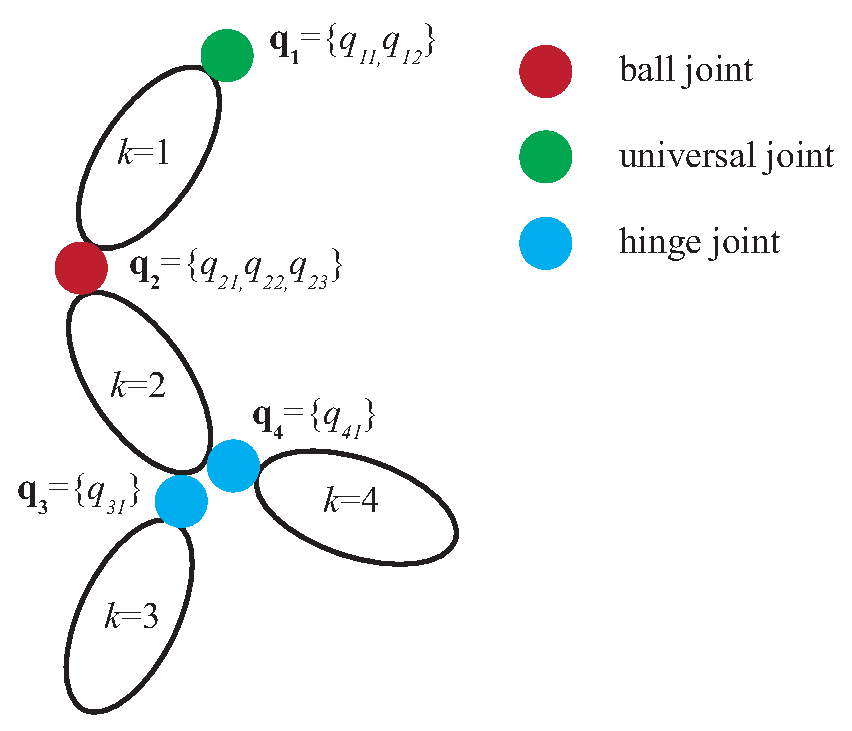
\includegraphics[width=2.1in]{example1_new.eps}
\end{center}
\caption{An articulated system.}
 \vspace{0pt}
\label{fig:example1}
\end{wrapfigure}

We list a few notations and definitions for an articulated rigid body system with $m$ rigid links. 
\begin{itemize}
\item $n(k)$ returns the number of DOFs in the parent joint of the link $k$. For example in Figure \ref{fig:example1}, $n(2) = 3$, $n(3) = 1$ etc. We denote the total number of DOFs in the system by $n$. \eg $n=7$ in Figure \ref{fig:example1}.
\item $p(k)$ returns the index of the parent link of link $k$. For
  example, $p(4) = 2$. $p(1,k)$ returns the indices of all the links in the chain from the root to the link $k$ (including $k$). For example, $p(1,4) = \{1,2,4\}$
\item $R_k$ is the local rotation matrix for the joint $k$ and depends only on the DOFs $\vc{q}_k$. $R^0_k$ is the chain of rotational transformations from the
  world frame to the local frame of the link $k$. Therefore, $R^0_k = R^0_{p(k)}R_k$.
\end{itemize}



\subsection{Cartesian and Generalized velocities}

For a single rigid body, \eqnref{vellin} and \eqnref{velang} describe the relation between the Cartesian velocities and the generalized velocities. 
For an articulated rigid body system, we use the same recipe as rigid body dynamics in \secref{rigidbodydyngen} and define the Jacobians for each rigid link that relate its respective Cartesian velocities to the generalized velocity of the entire system. 

We start with deriving the relation for the angular velocity. The angular velocity of link $k$ viewed in the world frame is:
\begin{eqnarray}
\nonumber
[\bm{\omega}_k] & = & \dot{R^0_k} {R^0_k}^T = \dot{(R^0_{p(k)}R_k)} (R^0_{p(k)}R_k)^T\\
\nonumber
& = & (\dot{R^0_{p(k)}}R_k + {R^0_{p(k)}}\dot{R_k})  R_k^T {R^0_{p(k)}}^T \\
\label{eq:angvelk_recursive}
& = & \dot{R^0_{p(k)}}{R^0_{p(k)}}^T + R^0_{p(k)} \left ( \dot{R_k} R_k^T \right ) {R^0_{p(k)}}^T \equiv [\bm{\omega}_{p(k)}] + R^0_{p(k)} [\hat{\bm{\omega}}_k] {R^0_{p(k)}}^T
%& = & [\bm{\omega}_{p(k)}] +  [R^0_{p(k)} \hat{\bm{\omega}}_k] = [\bm{\omega}_{p(k)} + R^0_{p(k)} \hat{\bm{\omega}}_k]
\end{eqnarray}
In the above equation, we define [$\hat{\bm{\omega}}_k] = \dot{R_k} R_k^T$ that denotes the angular velocity of the link $k$ in its \emph{parent} frame since the rotation matrix $R_k$ is the rotation of the rigid link $k$ with respect to its parent link $p(k)$. We can further write $\hat{\bm{\omega}}_k = \hat{J}_{\omega k} \dot{\vc{q}}_k$ where $\hat{J}_{\omega k}$ is the \emph{local} Jacobian matrix for the parent joint of link $k$ of size $3\times n(k)$. 

Using the property of skew symmetric matrix, $[R \bm{\omega}] = R [\bm{\omega}]
R^T$, we can express \eqnref{angvelk_recursive} in the vector form as:
\begin{eqnarray}
\label{eq:angvelk_iterative}
\nonumber
\bm{\omega}_k & = & \bm{\omega}_{p(k)} + R^0_{p(k)} \hat{J}_{\omega k} \dot{\vc{q}}_k\\
\nonumber
& = & \sum_{l \in p(1,k)} R^0_{p(l)} \hat{J}_{\omega l} \dot{\vc{q}}_l \mbox{\ \ (By unrolling the recursive definition)}\\
& \equiv & J_{\omega k}\dot{\vc{q}}
\end{eqnarray}
where the Jacobian $J_{\omega k}$ is:
\begin{equation}
\label{eq:angular_velocity_jac_link}
J_{\omega k} = \left ( \hat{J}_{\omega 1}\;\; \hdots\;\; R^0_{p(l)} \hat{J}_{\omega l} \;\;\hdots\;\; \vc{0} \;\;\hdots \right )
\end{equation}

Note that the zero matrices \vc{0} of size $3\times n(l)$ in $J_{\omega k}$ correspond to
joint DOFs $\vc{q}_l$ that are \emph{not} in the chain of transformations from the root to the
link $k$. 
Let us look at a couple of examples using the articulated
rigid body system in Figure \ref{fig:example1}:
\begin{eqnarray}
\bm{\omega}_1 &=& (\hat{J}_{\omega 1} \;\; \vc{0}
\;\;\vc{0}\;\;\vc{0}) \dot{\vc{q}}  \nonumber \\
\bm{\omega}_4 &=& (\hat{J}_{\omega 1} \;\; R^0_1\hat{J}_{\omega 2} \;\;
\vc{0} \;\;
R^0_2 \hat{J}_{\omega 4}) \dot{\vc{q}} \nonumber
\end{eqnarray}
Depending on the representation of the rotation $\vc{q}_k$,
$\hat{J}_{\omega k}$ can assume different values. For example, if the joint
between link $1$ and link $2$ in Figure \ref{fig:example1} is
represented as three Euler rotations, $R^{(x)}$, $R^{(y)}$, and
$R^{(z)}$ such that $R_2(\vc{q}_2)= R^{(x)}(q_{21}) R^{(y)}(q_{22}) R^{(z)}(q_{23})$, we have:
\begin{equation}
\hat{J}_{\omega 2} = 
\begin{pmatrix}
\begin{array}{c}
1\\
0\\
0
\end{array}
&
R^{(x)} \Bigg (
\begin{array}{c}
0\\
1\\
0
\end{array} 
\Bigg )
&
R^{(x)} R^{(y)}\Bigg (
\begin{array}{c}
0\\
0\\
1
\end{array} 
\Bigg )
\end{pmatrix}
\end{equation}
If the joint is represented as a quaternion or an
exponential map, $\hat{J}_{\omega k}$ does not have a simple symbolic form.

\ignorethis{
\begin{equation}
\label{eq:angular_velocity_link}
\bm{\omega}_k = (\vc{s}_1 \cdots \vc{s}_{np} \; R^0_{k-1} \vc{t}_1 \cdots
R^0_{k-1} \vc{t}_{nk}\; \vc{0} \cdots \vc{0}) \dot{\vc{q}} = J_{\omega k} \dot{\vc{q}}
\end{equation}
where $np$ is the number of DOFs in the parent chain and $nk$ is the
number of DOFs in the link $k$. 
}

Similarly, the linear velocity of the center of mass of the link $k$
can be expressed in terms of the generalized velocity: 
\begin{equation}
\label{eq:linear_velocity_link}
\vc{v}_k = J_{vk} \dot{\vc{q}}, \;\;\;\mathrm{where}\;\; J_{vk} = \frac{\partial \vc{x}_k}{\partial \vc{q}}=  \frac{\partial T^0_k
  \vc{c}_k}{\partial \vc{q}}.
\end{equation}
where the chain of homogeneous transformations from the world frame to the local
frame of link $k$ is denoted as $T^0_k$. Note that $T^0_k$ is
different from $R^0_k$ in that $T^0_k$ includes the translational
transformations. $\vc{c}_k$ denotes the center of mass of link $k$ in
its local frame.

We can concatenate the Cartesian velocities into a single vector $\vc{V}_k$ and denote the relation as:
\begin{eqnarray}
\label{eq:vel_relation_link}
\nonumber
\vc{V}_k & = & {J}_k \dot{\vc{q}}\\
\mbox{where } & & 
\vc{V}_k = \left (
\begin{array}{c}
\vc{v}_k\\
\bm{\omega}_k
\end{array}
\right ) \mbox{and\ }
{J}_k = \left (
\begin{array}{c}
J_{vk}\\
J_{\omega k}
\end{array}
\right ) 
\end{eqnarray}


\subsection{Equations of motion}
We now derive the equations of motion of an articulated rigid body system in generalized coordinates. The kinetic energy $T$ of the entire system can be expressed as the sum of kinetic energies of all the rigid links as $T=\sum_k T_k$. Therefore the equations of motion of the system can be computed as:
\begin{eqnarray}
\nonumber
\frac{d}{dt} \left ( \frac{\partial T}{\partial \dot{\vc{q}}} \right ) - \frac{\partial T}{\partial \vc{q}} & = & \frac{d}{dt} \left ( \frac{\partial \sum_k T_k}{\partial \dot{\vc{q}}} \right ) - \frac{\partial \sum_k T_k}{\partial \vc{q}}\\
\nonumber
& = & \sum_k \left ( \frac{d}{dt} \left ( \frac{\partial T_k}{\partial \dot{\vc{q}}} \right ) - \frac{\partial T_k}{\partial \vc{q}} \right )\\
\nonumber
& = & \sum_k \left ( \left( J_k^T M_{ck} J_k \right )\ddot{\vc{q}} + \left( J_k^T M_{ck} \dot{J}_k + J_k^T [\tilde{\bm{\omega}}_k]M_{ck} J_k \right )\dot{\vc{q}} \right )\\
& = &  \sum_k \left( J_k^T M_{ck} J_k \right )\ddot{\vc{q}} + \sum_k\left( J_k^T M_{ck} \dot{J}_k + J_k^T [\tilde{\bm{\omega}}_k]M_{ck} J_k \right )\dot{\vc{q}}
\end{eqnarray}
In deriving the above equation, we use the equations of motion in generalized coordinates for a single rigid body defined in \eqnref{dyngen_vec} subscripted by $k$ for the dynamics of $k^{th}$ link in the multibody system. The Jacobian $J_k$ for the $k^{th}$ link is defined in \eqnref{vel_relation_link}.



\section{Conversion between Cartesian and Generalized Coordinates}
In practice, we often want to use third-party rigid body simulators
rather than develop our own. There are a few widely used physics
engines that provide efficient, robust, and fairly accurate rigid body
simulation and collision handling. Open Dynamic Engine (ODE), PhysX, and
Bullet are perhaps the most popular free choices among game developers and
academic researchers. These commercial simulators use the maximal
representation rather than generalized coordinates
described above. That is, these simulators represent each link in the
articulated rigid body system as six DOFs,
leading to a redundant system with additional constraints between
links. A common practice is to develop control algorithms in
generalized coordinates and do forward simulation using a commercial
physics engine, such as ODE. This requires some conversion between
Cartesian and generalized coordinates.

\ignorethis{
\subsection{Definitions}
In the maximal coordinates, the state of an articulated rigid body
system can be expressed as $(\vc{x}_k, R_k, \vc{v}_k,
\boldsymbol{\bm{\omega}}_k)$, where $k = 1, \cdots, m$. Here $\vc{x}_k$ and
$R_k$ are the position and orientation of the rigid link $k$, and $(\vc{v}_k,
\boldsymbol{\bm{\omega}}_k)$ are the linear and angular velocity of the
rigid link $k$ viewed in the world frame. Similarly, we define the
Cartesian force and torque applied on rigid link $k$ as $(\vc{f}_k,
{\bm{\tau}}_k)$, both of which are expressed in the world
frame.
The same articulated rigid body system can be represented in
generalized coordinates. We define the generalized state as $(q_j,
\dot{q}_j)$, where $j = 1, \cdots, n$. The corresponding generalized
forces are then defined as $(Q_1, \cdots, Q_n)$.
}

\subsection{Velocity conversion}

We can concatenate all $2m$ Jacobian matrices corresponding to each link into a single Jacobian
that relates the generalized velocity to the Cartesian velocity of each
link:
\begin{equation}
\vc{V} \equiv 
\left(
\begin{array}{c}
\vc{v}_1 \\
\vdots \\
\vc{v}_m \\
\bm{\omega}_1 \\
\vdots \\
\bm{\omega}_m
\end{array}
\right) = 
\left (
\begin{array}{c}
J_{v1} \\
\vdots \\
J_{vm} \\
J_{\omega 1} \\
\vdots \\
J_{\omega m}
\end{array}
\right) 
\left(
\begin{array}{c}
\dot{\vc{q}}_1\\
\vdots \\
\dot{\vc{q}}_m
\end{array}
\right)  \equiv \left(
\begin{array}{c}
J_v\\
J_{\omega}
\end{array}
\right)\dot{\vc{q}} \equiv J \dot{\vc{q}}
\end{equation}

Typically, the Jacobian $J$ is full column rank because the
number of DOFs in the maximal representation is more than that in the
generalized representation, i.e $6m > n$. To compute $\dot{\vc{q}}$ from $\vc{V}$, we
will end up solving a over-constrained linear system. We can use
pseudo inverse of $J$ to compute $\dot{\vc{q}}$:
\begin{equation}
 \dot{\vc{q}} =  J^+\vc{V}
 \end{equation}
where the pseudo-inverse notation $J^+ = (J^TJ)^{-1}J^T$. 

Computing $J^+$ may be expensive for a system with many rigid links. 
Alternatively, we can rewrite the equation using the relative velocity between a child and a parent link expressed in the local
frame of the parent, instead of using velocities of each link
expressed in the world frame. As an example, we write the simplified expression for the angular velocity of link $k$ using \eqnref{angvelk_iterative} as: 
\begin{eqnarray}
\nonumber
\bm{\omega}_k - \bm{\omega}_{p(k)} & = & R^0_{p(k)}\hat{\bm{\omega}}_k = R^0_{p(k)}\hat{J}_{\omega k} \dot{\vc{q}}_k \\
\Rightarrow \left ( -\vc{I}_3\;\; \vc{I}_3 \right ) 
\left ( 
\begin{array}{c}
\bm{\omega}_{p(k)}\\
\bm{\omega}_k
\end{array}
\right ) & = & R^0_{p(k)}\hat{J}_{\omega k} \dot{\vc{q}}_k
\end{eqnarray}

%\begin{pmatrix}
%\vc{0}  &                    &  &\\
%        & \ddots             &  & \\
%        &                    & R^0_{p(k)}\hat{J}_{\omega k} & \\
%        &                    &  & \ddots & \\
%        &                    &   &     & \vc{0}
%\end{pmatrix} 

Combining these equations for all the links, we get:
\begin{eqnarray}
\label{eq:jacsplit}
\nonumber
D \bm{\omega} = D J_{\omega} \dot{\vc{q}} & = & \mbox{blockdiag}(\hat{J}_{\omega 1},\hdots,R^0_{p(m)}\hat{J}_{\omega m})\dot{\vc{q}}\\
\nonumber
& = & \mbox{blockdiag}(\vc{I}_3,\hdots,R^0_{p(m)})\mbox{blockdiag}(\hat{J}_{\omega 1},\hdots,\hat{J}_{\omega m})\dot{\vc{q}}\\
& \equiv & \hat{R} \hat{J}_{\omega}\dot{\vc{q}}
\end{eqnarray}
where $D$ is a constant matrix that encodes the connectivity between links. For example, matrix $D$ for the system in Figure \ref{fig:example1} looks
like:
\begin{equation}
D =
\left (
\begin{array}{cccc}
\vc{I}_{3}  & \vc{0} & \vc{0} & \vc{0}\\
-\vc{I}_{3} & \vc{I}_{3}  & \vc{0} & \vc{0}\\
\vc{0} & -\vc{I}_{3} & \vc{I}_{3}  & \vc{0}\\
\vc{0} & -\vc{I}_{3} & \vc{0} & \vc{I}_{3}\\
\end{array}
\right )  
\end{equation}
The relation between $\hat{J}_{\omega}$ and $J_{\omega}$ follows from \eqnref{jacsplit}:
\begin{equation}
\label{eq:jacbodyhat}
\hat{J}_{\omega} = \hat{R}^T D J_{\omega}
\end{equation}
The matrix $\hat{J}_{\omega}$ being block diagonal is much sparser as compared to ${J}_{\omega}$. For rotational DOFs, it is sufficient to invert only $J_{\omega}$. Therefore, we can compute $\dot{\vc{q}}$ as:
\begin{eqnarray}
\nonumber
 \dot{\vc{q}} & = & J_{\omega}^+ \bm{\omega}\\
 \nonumber
 & = &  \hat{J}_{\omega}^+ \hat{R}^T D\bm{\omega}\\
 & = & \mbox{blockdiag}\left(\hat{J}_{\omega 1}^+,\hdots,\hat{J}_{\omega m}^+\right ) \mbox{blockdiag}\left(\vc{I}_3,\hdots,{R^0_{p(m)}}^T\right ) D\bm{\omega}
\end{eqnarray}
Therefore, we see that the problem of computing pseudo-inverse of a matrix $J_{\omega}$ is reduced to computing $m$ pseudo-inverses of much smaller constant-sized matrices $\hat{J}_{\omega k}$.


\subsection{Force conversion}
The relation between the Cartesian force and the generalized force can
be found in \eqnref{virtual_work}:
\begin{equation}
\label{eq:force_conversion}
\vc{Q} = \sum_i {J^{'}_{vi}}^T \vc{f}_i + \sum_k J_{\omega k}^T \bm{\tau}_k = 
\left (
\begin{array}{cc}
{J^{'}_{v}}^T & J_\omega^T
\end{array}
\right)
\left(
\begin{array}{c}
\vc{f} \\
\bm{\tau}
\end{array}
\right) 
, \;\;\;\mathrm{where}\;\;
J^{'}_{vi} = \frac{\partial \vc{r}_i}{\partial \vc{q}}
\end{equation}
where $\vc{r}_i$ is the point of application of the Cartesian force
$\vc{f}_i$ expressed in the world frame. 

\paragraph{Note.} Body torque $\bm{\tau}_k$ is the torque
applied on link $k$ in the world frame and does \emph{not} include the torque induced by the linear forces $\vc{f}_i$. 
However, the definition for torque in \eqnref{summary_dynamics} \emph{includes} the torque $[\vc{r}_i-\vc{x}_i] \vc{f}_i$ due to each force $\vc{f}_i$ ($\vc{x}_i$ is the COM of the link $i$). As a result, the linear Jacobian $J_{v}$ in \eqnref{summary_dynamics} is defined for the COM of the respective rigid link and $J^{'}_{v}$ in \eqnref{force_conversion} is defined for the point of application of the force. It is easy to verify that ${J^{'}_{vi}}^T\vc{f}_i = J_{vi}^T\vc{f}_i + J_{\omega i}^T[\vc{r}_i-\vc{x}_i] \vc{f}_i$.
%However, for the sake of clarity, we use the new definition of the Jacobian in \eqnref{force_conversion} and abuse the notation by denoting it by $J_v$.

Often many controllers (such as a tracking controller) find it convenient to compute the Cartesian-space \emph{joint torques} in the local frame of the parent link rather than \emph{body torques} in the world frame. Joint torque $\hat{\bm{\tau}}_k$ in the frame of parent link $p(k)$ is defined such that positive torque in the world frame $R^0_{p(k)}\hat{\bm{\tau}}_k$ is applied to the link $k$ and negative torque $-R^0_{p(k)}\hat{\bm{\tau}}_k$ is applied to the parent link $p(k)$. Therefore, the body torque $\bm{\tau}_k$ applied to the link $k$ can be written in terms of the joint torques as $\bm{\tau}_k = R^0_{p(k)}\hat{\bm{\tau}}_k - \sum_l R^0_{k} \hat{\bm{\tau}}_l$, $\forall l:k=p(l)$. Collecting the body torques for all the rigid links in the vector $\bm{\tau}$, the relation between the body torques and the joint torques can be defined as:
\begin{eqnarray}
\label{eq:torquesbodyhat}
\bm{\tau} & = & D^T \hat{R} \hat{\bm{\tau}} = (\hat{R}^T D)^T \hat{\bm{\tau}}
\end{eqnarray}
where $\hat{R}, D$ are defined in \eqnref{jacbodyhat}. We now substitute \eqnref{torquesbodyhat} in \eqnref{force_conversion} and get:
\begin{eqnarray}
\nonumber
\vc{Q} & = & 
\left (
\begin{array}{cc}
{J^{'}_{v}}^T & J_\omega^T
\end{array}
\right )
\begin{pmatrix}
\vc{f} \\
(\hat{R}^T D)^T \hat{\bm{\tau}}
\end{pmatrix}
 \\
\nonumber
& = & 
\left (
\begin{array}{cc}
{J^{'}_{v}}^T & (\hat{R}^T D J_\omega)^T
\end{array}
\right )
\left (
\begin{array}{c}
\vc{f} \\
\hat{\bm{\tau}}
\end{array}
\right )
\\
& = & 
\left (
\begin{array}{cc}
{J^{'}_{v}}^T & \hat{J}_\omega^T
\end{array}
\right )
\left (
\begin{array}{c}
\vc{f} \\
\hat{\bm{\tau}}
\end{array}
\right ) \mbox{\ \ (Using \eqnref{jacbodyhat})}
\end{eqnarray}


%\section{Recursive Inverse and Forward Dynamics}
\section{Introduction}
If you have not read the excellent SIGGRAPH course notes on
physics-based animation by Witkin and Baraff, you can stop reading
further right now. Go look for those notes at
{\tt http://www.cs.cmu.edu/\textasciitilde baraff/sigcourse/} and come back when
you fully understand everything in the notes.

If you are still reading this document, you probably fit the following
profile. You are a computer scientist with no mechanical engineering
background and minimal training in physics in high school but you are
seriously interested in physics-based character animation. You have
read Witkin and Baraff's SIGGRAPH course notes a few times but don't
know where to go from simulating rigid bodies to human figures. You
have played with some commercial physics engines like ODE (Open
Dynamic Engine), PhysX, Havok, or Bullet, but you wish to
simulate human behaviors more interesting than ragdoll effects.

Physics-based character animation consists of two parts: simulation
and control. This document focuses on the simulation part. It's quite
likely that you do not need to understand how underlying simulation
works if your control algorithm is simple enough. However, complex
human behaviors often require sophisticated controllers that exploit
the dynamics of a multibody system. A good understanding of multibody
dynamics is paramount for designing effective controllers.

There are many ways to learn multibody dynamics. Reading a textbook
on this topic or taking a course from the mechanical engineering
department will both do the job. However, if you only want to learn
the minimal set of multibody dynamics necessary to jump start your
research in physics-based character animation, this document might be
what you are looking for. In particular, this document attempts to
answer the following questions.

\begin{itemize}
\item I know how to derive the equations of motion for one rigid body
  and I have seen people use the following equations for articulated
  rigid bodies, but I don't know how they are derived.
\begin{equation}
M(\vc{q}) \ddot{\vc{q}} + C(\vc{q}, \dot{\vc{q}})  = \vc{Q} \nonumber
\end{equation}

\item I have seen Lagrangian equation in the following form before, but I
  don't know how it is related to the equations of motion above.
\begin{equation}\label{eq:lagrangian_dyn}
    \frac{d}{dt} \left( \frac{\partial \sKinetics_i}{\partial
    \dot{\vJoint}} \right) - \frac{\partial \sKinetics_i}{\partial
    \vJoint} - \vc{Q} = 0 \nonumber
\end{equation}

\item I use generalized coordinates to compute the control forces, how do I convert them to Cartesian forces such that I can use simulators like ODE, PhysX, or Bullet which represent rigid bodies in the maximal coordinates?

\item I heard inverse dynamics can be computed recursively to improve performance. How does that work?
\end{itemize}


\newpage
\section{Lagrangian Dynamics}
\label{sec:lagrangian}
Articulated human motions can be described by a set of dynamic
equations of motion of multibody systems. Since the direct application
of Newton's second law becomes difficult when a complex human skeleton
is considered, we use \emph{Lagrange's equations} derived from
\emph{D'Alembert's principle} to describe the dynamic of the
motions. To simplify the math, let's temporarily imagine the entire
human skeleton consists of a collection of particles
$\{\vGlobalPoint_1, \vGlobalPoint_2, \ldots,
\vGlobalPoint_{\sNumParticle}\}$.  Each particle, $\vGlobalPoint_i$,
is defined by Cartesian coordinates that describe the translation with
respective to the world coordinates.  We can represent
$\vGlobalPoint_i$ by a set of \emph{generalized coordinates} that
indicate the joint configuration of the human skeleton:
\begin{equation}\label{eq:general_coord}
    \vGlobalPoint_i = \vGlobalPoint_i(\sJoint_{1},
\sJoint_{2}, \ldots, \sJoint_{\sNumJoint}, t)
\end{equation}
where $t$ is the time and $\sJoint_j$ is a joint degree of freedom (DOF) in
the skeleton.

The virtual displacement $\delta \vGlobalPoint_i$ refers to an
infinitesimal change in the system coordinates such that the
constraint remains satisfied. In the context of human skeleton, the
system coordinates are the generalized coordinates $\sJoint_j$ and the
constraint manifold lies in the Cartesian space. The virtual
displacement $\delta \vGlobalPoint_i$ is a tangent vector to the
constraint manifold at a fixed time, written as
\begin{equation}\label{eq:virtual_displace}
    \delta \vGlobalPoint_i = \sum_j \frac{\partial \vGlobalPoint_i}{\partial
    \sJoint_j}\delta \sJoint_j
\end{equation}

We can now write the virtual work done by a force $\vForce{i}$ acting on particle
$\vGlobalPoint_i$ as
\begin{equation}\label{eq:virtual_work}
  \vc{f}_{i} \cdot  \delta \vc{r}_i = \vc{f}_{i} \cdot  \sum_j \frac{\partial \vc{r}_i}{\partial
    q_j}\delta q_j \equiv \sum_j Q_{ij} \delta q_j = \vc{Q}_i \cdot \delta \vc{q}
\end{equation}
where $Q_{ij} = \left ( \frac{\partial \vc{r}_i}{\partial q_j} \right )^T \vc{f}_i$ is defined as the component of the \emph{generalized force}
associated with coordinate $q_j$. In vector form, $\vc{Q}_i$ is the generalized force corresponding to the Cartesian force $\vc{f}_i$ with the relation $\vc{Q}_i = J_i^T \vc{f}_i$, where $J_i$ is the Jacobian matrix with the $j^{th}$ column defined as $\frac{\partial \vc{r}_i}{\partial q_j}$.

From D'Alembert's principle, we know that the sum of the differences
between the forces acting on a system and the inertial force of the
system along any virtual displacement consistent with the constraints
of the system, is zero. Therefore, the virtual work at $\vGlobalPoint_i$ can be written as
\begin{equation}\label{eq:inertial_work}
  \delta \sWork_i = \vForce{i} \cdot  \delta \vGlobalPoint_i =
  \sInfMass_i \ddot{\vGlobalPoint}_i \cdot \delta \vGlobalPoint_i =
  \sum_j \sInfMass_i \ddot{\vGlobalPoint}_i \cdot
    \frac{\partial \vGlobalPoint_i}{\partial \sJoint_j} \delta \sJoint_j
\end{equation}
where $\sInfMass_i$ is the infinitesimal mass associated with
$\vGlobalPoint_i$. The component of inertial force associated with
$\sJoint_j$ can be written as
\begin{equation}
\label{eq:inertia_force}
  \sInfMass_i \ddot{\vGlobalPoint}_i \cdot \frac{\partial \vGlobalPoint_i}{\partial \sJoint_j} =
  \frac{d}{dt} \left( \sInfMass_i \dot{\vGlobalPoint}_i \cdot \frac{\partial
  \vGlobalPoint_i}{\partial \sJoint_j} \right) - \sInfMass_i
\dot{\vGlobalPoint}_i \cdot \frac{d}{dt} \left( \frac{\partial
    \vGlobalPoint_i}{\partial \sJoint_j} \right) 
\end{equation}

Now let us consider the velocity of $\vGlobalPoint_i$ in terms of
joint velocity $\dot{\sJoint}_j$
\begin{equation}
\label{eq:velocity}
\dot{\vGlobalPoint}_i = \sum_j \frac{\partial
  \vGlobalPoint_i}{\partial \sJoint_j} \dot{\sJoint}_j
\end{equation}
from which we derive the following two identities:
\begin{eqnarray}
\frac{\partial \dot{\vGlobalPoint}_i}{\partial \dot{\sJoint}_j} &=&
\frac{\partial \vGlobalPoint_i}{\partial \sJoint_j}  \\
\frac{\partial \dot{\vGlobalPoint}_i}{\partial \sJoint_j} &=&
\sum_k \frac{\partial^2 \vGlobalPoint_i}{\partial \sJoint_j \partial
  \sJoint_k} \dot{\sJoint}_k = \frac{d}{dt} \frac{\partial \vGlobalPoint_i}{\partial \sJoint_j}
\end{eqnarray}

Using these two identities, we rewrite \eqnref{inertia_force} as
\begin{equation}
\label{eq:inertia_force2}
\sInfMass_i \ddot{\vGlobalPoint}_i \cdot \frac{\partial \vGlobalPoint_i}{\partial \sJoint_j}   = \frac{d}{dt} \left ( \frac{\partial}{\partial \dot{\sJoint}_j} \left( \frac{1}{2} \sInfMass_i \dot{\vGlobalPoint}_i^{T} \dot{\vGlobalPoint}_i\right) \right)
   - \frac{\partial}{\partial \sJoint_j} \left( \frac{1}{2} \sInfMass_i \dot{\vGlobalPoint}_i^{T} \dot{\vGlobalPoint}_i \right)
\end{equation}

We can denote the kinetic energy of $\vGlobalPoint_i$ as
\begin{equation}\label{eq:kinetic_energy}
    \sKinetics_i = \frac{1}{2} \sInfMass \dot{\vGlobalPoint}_i^{T}
    \dot{\vGlobalPoint}_i,
\end{equation}
and rewrite \eqnref{inertia_force2} as
\begin{equation}\label{eq:inertia_kinetic}
    \sInfMass_i \ddot{\vGlobalPoint}_i \cdot \frac{\partial \vGlobalPoint_i}{\partial
    \sJoint_j} = \frac{d}{dt} \left( \frac{\partial \sKinetics_i}{\partial
    \dot{\sJoint}_j}\right) - \frac{\partial \sKinetics_i}{\partial \sJoint_j}
\end{equation}

Combining the definition of generalized force (\eqnref{virtual_work}), D'Alembert's principle (\eqnref{inertial_work}), and the generalized inertial force (\eqnref{inertia_kinetic}), we arrive at the following equation:
\begin{equation}\label{eq:dynamic_equil}
    \left ( \frac{d}{dt} \left( \frac{\partial \sKinetics_i}{\partial \dot{\sJoint}_j} \right) - \frac{\partial \sKinetics_i}{\partial
    \sJoint_j}\right ) \delta \sJoint_j = Q_{ij} \delta
    \sJoint_j
\end{equation}

If the set of generalized coordinates $\sJoint_j$ is linearly
independent, \eqnref{dynamic_equil} leads to
\emph{Lagrangian equation}:
\begin{equation}\label{eq:lagrangian_dyn2}
    \frac{d}{dt} \left( \frac{\partial \sKinetics_i}{\partial
    \dot{\sJoint}_j} \right) - \frac{\partial \sKinetics_i}{\partial
    \sJoint_j} - Q_{ij} = 0
\end{equation}

\paragraph{Equations of Motion in Vector Form.} \eqnref{lagrangian_dyn2} is the equation of motion for one generalized coordinate in a
multibody system. We can combine $\sNumJoint$  scalar equations into
the familiar vector form
\begin{equation}\label{eq:lagrangian_vector}
M(\vc{q}) \ddot{\vc{q}} + C(\vc{q}, \dot{\vc{q}}) = \vc{Q} 
\end{equation}
where $M(\vc{q})$ is the mass matrix, $C(\vc{q}, \dot{\vc{q}})$ is the
Coriolis and centrifugal term of the equation of motion, and $\vc{Q}$
is the vector of generalized forces for all the degrees of freedom
(DOFs) in the system. $M$ only depends on $\vc{q}$ and $C$ depends
quadratically on $\dot{\vc{q}}$.

How do we derive $M$ and $C$ from \eqnref{lagrangian_dyn2}?
Let us go back to the velocity of one particle $\vGlobalPoint_i$:
\begin{equation}
\dot{\vGlobalPoint}_i = \sum_j \frac{\partial
  \vGlobalPoint_i}{\partial \sJoint_j} \dot{\sJoint}_j = J_i(\vc{q}) \dot{\vc{q}}
\end{equation}
where $J_i$ denotes the Jacobian of $\vGlobalPoint_i$. By summing up
all the particles in the system, the kinetic
energy of the system can then be expressed as
\begin{equation}
\label{eq:kinetic_vector}
T = \sum_i T_i = \sum_i \frac{1}{2}  \sInfMass \dot{\vGlobalPoint}_i^{T}
    \dot{\vGlobalPoint}_i = \sum_i \frac{1}{2}  \sInfMass (J_i
    \dot{\vc{q}})^T(J_i \dot{\vc{q}}) = \frac{1}{2} \dot{\vc{q}}^T
    (\sum_i \sInfMass J_i^TJ_i) \dot{\vc{q}} = \frac{1}{2}
    \dot{\vc{q}}^T M(\vc{q}) \dot{\vc{q}}
\end{equation}
where we define the mass matrix, $M(\vc{q}) = \sum_i \sInfMass
J_i^TJ_i$, and will shortly show it is indeed the mass matrix in
\eqnref{lagrangian_vector}.

From \eqnref{kinetic_vector}, we can derive the derivative
terms to construct the Lagrange's equation (\eqnref{lagrangian_dyn2}):
\begin{equation}
\label{eq:lagrangian_vector2}
\frac{d}{dt}\frac{\partial T}{\partial \dot{\vc{q}}} - \frac{\partial
  T}{\partial \vc{q}} = M\ddot{\vc{q}} + \dot{M} \dot{\vc{q}} - \frac{1}{2}\dot{\vc{q}}^T \left ( \frac{\partial M}{\partial \vc{q}} \right )^T \dot{\vc{q}} \equiv M
\ddot{\vc{q}} + C(\vc{q}, \dot{\vc{q}})
\end{equation}

Comparing \eqnref{lagrangian_vector2} to \eqnref{lagrangian_vector},
we confirm that the mass matrix is identical in both equations. $C$ is
the Coriolis and centrifugal term in \eqnref{lagrangian_vector} and is
defined as $C = \dot{M} \dot{\vc{q}} - \frac{1}{2}\left( \frac{\partial M}{\partial  \vc{q}} \dot{\vc{q}} \right)^T \dot{\vc{q}}$. 

\paragraph{Note.} In the second term of $C$, we introduce tensor notation $\frac{\partial M}{\partial \vc{q}}$, which implies that the $j^{th}$ element of the tensor $\frac{\partial M}{\partial \vc{q}}$ is the matrix $\frac{\partial M}{\partial {q}_j}$. Note that, in general, the quantity with notation $\frac{\partial M}{\partial \vc{q}} \dot{\vc{q}}$ is \textbf{\emph{not}} equal to $\dot{M}$. This is because, the $j^{th}$ column of the matrix $\frac{\partial M}{\partial \vc{q}} \dot{\vc{q}}$ is the vector $\frac{\partial M}{\partial q_j} \dot{\vc{q}}$ or $\sum_k \frac{\partial (M)_k}{\partial q_j} \dot{{q}_k}$, where the notation $(A)_j$ denotes the $j^{th}$ column of the matrix $A$. In contrast, the $j^{th}$ column of the matrix $\dot{M}$ is $\sum_k \frac{\partial (M)_j}{\partial q_k} \dot{{q}_k}$.

Once we know how to compute the mass matrix, Coriolis and centrifugal
terms, and generalized forces, we can compute the acceleration in
generalized coordinates, $\ddot{\vc{q}}$, for forward
dynamics. Conversely, if we are given $\ddot{\vc{q}}$ from a motion
sequence, we can use these equations of motion to derive generalized
forces for inverse dynamics. 

The above formulation is convenient for a system consisting of finite
number of mass points. However, for a dynamic system that consists of
rigid bodies, there are infinitely many points contained in each rigid
body making the above formulation intractable. In the following two
sections, we view a rigid body as a continuum and derive compact
equations of motions in both Cartesian coordinates and generalized
coordinates.

\newpage
\section{Rigid Body Dynamics: Newton-Euler equations}
This section describes the familiar Newton-Euler equations of rigid
body dynamics. We begin with the momenta of the rigid body whose mass,
position of the center of mass (COM), orientation, linear velocity of
the COM, and angular velocity are $m$, $\vc{x}$, $R$, $\vc{v}$, and
$\bm{\omega}$ respectively (same as defined in Witkin and Baraff's
course notes). The linear momentum \vc{p} is computed as:
\begin{eqnarray}
\vc{p} &=& \sum_i \vc{p}_i = \sum_i \sInfMass \dot{\vGlobalPoint}_i = \sum_i  \sInfMass (\vc{v} + \bm{\omega}
    \times \vc{r}_i') \nonumber \\
 &=& m \vc{v}
\end{eqnarray}
where $\vc{r}_i' = \vc{r}_i - \vc{x}$. Because $\sum_i \sInfMass
\vc{r}_i' = \vc{0}$ (property of the COM), the second term vanishes. The angular momentum \vc{L} about the COM is computed as:
\begin{eqnarray}
\nonumber
\vc{L} & = & \sum_i \vc{L}_i  = \sum_i \vc{r}_i' \times \vc{p}_i\\
\nonumber
& = & \sum_i \sInfMass \vc{r}_i' \times (\vc{v} + \bm{\omega} \times \vc{r}_i')\\
&= & \vc{0} + \sum_i \sInfMass [\vc{r}_i'][\bm{\omega}]\vc{r}_i' = \left ( \sum_i -\sInfMass [\vc{r}_i'][\vc{r}_i'] \right )\bm{\omega}
\end{eqnarray}
The notation $[\vc{a}] \vc{b}$ denotes the cross product $\vc{a}\times \vc{b}$ with $[\vc{a}]$ being the skew-symmetric matrix corresponding to the vector $\vc{a}$:
\begin{equation}
[\vc{a}] = 
\begin{pmatrix}
0 & -a_3 & a_2\\
a_3&  0 & -a_1\\
-a_2 & a_1 & 0
\end{pmatrix}
\end{equation}
Therefore the following identities hold: $[\vc{a}]\vc{b} = -[\vc{b}]\vc{a}$ and $[\vc{a}]^T = -[\vc{a}]$.

Now recall the inertia tensor about the COM defined in Witkin and
Baraff's course notes: $I_c = \sum_i \sInfMass ((\vc{r}_i'^T
\vc{r}_i')\vc{I}_3 - \vc{r}_i' \vc{r}_i'^T)$, where $\vc{I}_3$ is the $3\times 3$
identity matrix. We can easily show that
$I_c = \sum_i -\sInfMass [\vc{r}_i'][\vc{r}_i']$ by verifying the
identity $-[\vc{a}][\vc{a}] = (\vc{a}^T\vc{a}) \vc{I}_3  -
\vc{a}\vc{a}^T$. As a result, we write the angular momentum of a rigid body as:
\begin{equation}
\vc{L} = I_c \bm{\omega}
\end{equation}
Note that the inertia tensor can be written as $I_c = RI_0R^T$, where $R$ is the rotation matrix corresponding to the orientation of the body and $I_0$ is the constant inertia tensor defined at zero rotation. The angular velocity in the skew-symmetric form is related to the rotation matrix $R$ as $[\bm{\omega}] = \dot{R}R^T$. Also $[\bm{\omega}]^T = -[\bm{\omega}]$.

Now, the dynamics of a rigid body can be written as $\vc{f} = \dot{\vc{p}} \mbox{,\ } \bm{\tau} = \dot{\vc{L}}$. The equations corresponding to the linear force can be evaluated as:
\begin{eqnarray}
\label{eq:force}
\vc{f} & = & \dot{\vc{p}} = m \dot{\vc{v}}
\end{eqnarray}
The equations corresponding to the torque can be evaluated as:
\begin{eqnarray}
\label{eq:torque}
\nonumber
\bm{\tau} & = & \dot{\vc{L}} = \dot{(I_c \bm{\omega})} \\
\nonumber
& = & I_c\dot{\bm{\omega}} + \dot{(RI_0 R^T)}\bm{\omega} = I_c\dot{\bm{\omega}} + \dot{R}I_0 R^T\bm{\omega} + R I_0 \dot{R}^T\bm{\omega}\\
\nonumber
& = & I_c\dot{\bm{\omega}} + \dot{R}R^T I_c \bm{\omega} + I_c (\dot{R}R^T)^T\bm{\omega} \\
& = & I_c\dot{\bm{\omega}} + [\bm{\omega}]I_c \bm{\omega} - I_c[\bm{\omega}]\bm{\omega} = I_c\dot{\bm{\omega}} + \bm{\omega} \times I_c \bm{\omega}
\end{eqnarray}

Combining \eqnref{force} and \eqnref{torque}, we arrive at the
Newton-Euler equations:
\begin{equation}
\label{eq:newtoneuler}
\left(
\begin{array}{cc}
m\vc{I}_3 & \vc{0} \\
\vc{0} & I_c 
\end{array}
\right)
\left(
\begin{array}{c}
\dot{\vc{v}} \\
\dot{\bm{\omega}} 
\end{array}
\right) +
\left(
\begin{array}{c}
\vc{0}  \\
\bm{\omega} \times I_c \bm{\omega} 
\end{array}
\right) = 
\left(
\begin{array}{c}
\vc{f} \\
\bm{\tau} 
\end{array}
\right)
\end{equation}


\newpage
\section{Rigid Body Dynamics: Lagrange's equations}
\label{sec:rigidbodydyngen}
The Newton-Euler equations are defined in terms of velocities instead of position and orientation. We now derive the equations in generalized coordinates \vc{q} that define the position and orientation. The first three coordinates are the same as the position of COM. The next three represent the rotation of the rigid body such as an exponential map or three Euler angles (or four coordinates can be used for a quaternion).

We start by computing the kinetic energy of the rigid body:
\begin{eqnarray}
\label{eq:rigid_kinetic}
T &=& \sum_i T_i = \sum_i \frac{1}{2}  \sInfMass \dot{\vGlobalPoint}_i^{T}
    \dot{\vGlobalPoint}_i = \sum_i \frac{1}{2}  \sInfMass (\vc{v} + \bm{\omega}
    \times \vc{r}_i')^T (\vc{v} + \boldsymbol{\bm{\omega}}
    \times \vc{r}_i') \nonumber \\
 &=& \sum_i \frac{1}{2}  \sInfMass (\vc{v}^T\vc{v} +
    \vc{v}^T [\bm{\omega}] \vc{r}_i' + \vc{r}_i'^T [\bm{\omega}]^T \vc{v} +
    \vc{r}_i'^T [\bm{\omega}]^T [\bm{\omega}] \vc{r}_i')
\end{eqnarray}
Because $\sum_i \sInfMass
\vc{r}_i' = \vc{0}$, the second term and the third term in \eqnref{rigid_kinetic} vanish. Using the identity $[\bm{\omega}]\vc{r}_i' =
-[\vc{r}_i']\bm{\omega}$, we can rewrite \eqnref{rigid_kinetic}
as:
\begin{eqnarray}
\nonumber
T & = & \frac{1}{2} m \vc{v}^T\vc{v} + \frac{1}{2} \bm{\omega}^T \left ( \sum_i -\sInfMass
 [\vc{r}_i'][\vc{r}_i'] \right ) \bm{\omega}\\
 & = & \frac{1}{2} m \vc{v}^T\vc{v} + \frac{1}{2} \bm{\omega}^T I_c \bm{\omega}
\end{eqnarray}
The kinetic energy of a rigid body can be written in its vector form:
\begin{eqnarray}
\label{eq:kinetic_vec}
T &=& \frac{1}{2} (\vc{v}^T \;\; \bm{\omega}^T)
\left(
\begin{array}{cc}
m\vc{I}_3 & \vc{0} \\
\vc{0} & I_c
\end{array}
\right)
\left(
\begin{array}{c}
\vc{v} \\
\bm{\omega} 
\end{array}
\right)
 \equiv \frac{1}{2}\vc{V}^T M_c \vc{V}
\end{eqnarray}
where $\vc{V} = (\vc{v}^T,\bm{\omega}^T)^T$, $M_c = \mbox{blockdiag}(m\vc{I}_3,I_c)$. We now relate the velocities in the Cartesian space $\vc{V}$ to the generalized velocities $\dot{\vc{q}}$. Let $\vc{x}(\vc{q})$ and $R(\vc{q})$ represent the position of the COM and the rotation matrix of the rigid body. The linear velocity of the COM is computed as:
\begin{eqnarray}
\label{eq:vellin}
\vc{v} = \dot{\vc{x}}(\vc{q}) = \frac{\partial \vc{x}}{\partial \vc{q}} \dot{\vc{q}} \equiv J_v \dot{\vc{q}}
\end{eqnarray}
The angular velocity is computed as:
\begin{eqnarray}
\nonumber
[\bm{\omega}] & = & \dot{R}(\vc{q})R^T(\vc{q}) \\
\label{eq:Jaccolj}
& = & \sum_j \frac{\partial R}{\partial q_j}R^T \dot{q}_j \equiv \sum_j [\vc{j}_{j}] \dot{q}_j
\end{eqnarray}
$\frac{\partial R}{\partial q_j}R^T$ is always a skew-symmetric matrix that we represent as $[\vc{j}_{j}]$ (skew-symmetric form of the vector $\vc{j}_j$). $\bm{\omega}$ can now be represented in the vector form as:
\begin{equation}
\label{eq:velang}
\bm{\omega} = J_{\omega} \dot{\vc{q}}
\end{equation}
where $\vc{j}_{j}$ is the $j^{th}$ column of the matrix $J_{\omega}$.

Using \eqnref{vellin} and \eqnref{velang}, we can write:
\begin{equation}
\label{eq:velcartall}
\vc{V} = \left(
\begin{array}{c}
J_v \\
J_{\omega}
\end{array}
\right) \dot{\vc{q}} \equiv J(\vc{q})\dot{\vc{q}}
\end{equation}
Substituting the above in \eqnref{kinetic_vec}, we get:
\begin{equation}
T = \frac{1}{2}\dot{\vc{q}}^T J^T M_c J \dot{\vc{q}}
\end{equation}

Using the recipe for Lagrangian dynamics in \eqnref{lagrangian_dyn2}, we first compute $\frac{\partial T}{\partial \dot{q}_j}$ as:
\begin{eqnarray}
\nonumber
\frac{\partial T}{\partial \dot{q}_j} & = & \frac{1}{2}\dot{\vc{q}}^T J^T M_c (J)_j + \frac{1}{2} (J)_j^T M_c J \dot{\vc{q}}\\
 & = & (J)_j^T M_c J \dot{\vc{q}}
\end{eqnarray}
where the notation $(A)_j$ denotes the $j^{th}$ column of the matrix A. The term $\frac{d}{dt} \left( \frac{\partial T}{\partial \dot{q}_j} \right )$ is computed as:
\begin{eqnarray}
\label{eq:lagterm1}
\frac{d}{dt} \left ( \frac{\partial T}{\partial \dot{q}_j} \right ) & = & (J)_j^T M_c J \ddot{\vc{q}} + (J)_j^T M_c \dot{J} \dot{\vc{q}} + (J)_j^T \dot{M}_c J \dot{\vc{q}} + \dot{(J)}_j^T M_c J \dot{\vc{q}}
\end{eqnarray}
Now we evaluate the term $\frac{\partial T}{\partial q_j}$:
\begin{eqnarray}
\nonumber
\frac{\partial T}{\partial q_j} & = & \frac{1}{2}\dot{\vc{q}}^T J^T M_c \frac{\partial J}{\partial q_j} \dot{\vc{q}} + \frac{1}{2}\dot{\vc{q}}^T J^T \frac{\partial M_c}{\partial q_j} J \dot{\vc{q}} + \frac{1}{2}\dot{\vc{q}}^T \frac{\partial J^T}{\partial q_j} M_c J \dot{\vc{q}}\\
\label{eq:lagterm2}
& = & \dot{\vc{q}}^T \frac{\partial J^T}{\partial q_j} M_c J \dot{\vc{q}} + \frac{1}{2}\dot{\vc{q}}^T J^T \frac{\partial M_c}{\partial q_j} J \dot{\vc{q}}
\end{eqnarray}
Using the above equations, we write:
\begin{eqnarray}
\label{eq:lageqn_j}
\nonumber
\frac{d}{dt} \left ( \frac{\partial T}{\partial \dot{q}_j} \right ) - \frac{\partial T}{\partial q_j} & = & (J)_j^T M_c J \ddot{\vc{q}} + (J)_j^T M_c \dot{J} \dot{\vc{q}} + (J)_j^T \dot{M}_c J \dot{\vc{q}} - \frac{1}{2}\dot{\vc{q}}^T J^T \frac{\partial M_c}{\partial q_j} J \dot{\vc{q}} \\ & & + \left ( \dot{(J)}_j^T M_c J \dot{\vc{q}}  - \left( \frac{\partial J}{\partial q_j} \dot{\vc{q}}\right)^T M_c J \dot{\vc{q}} \right )
\end{eqnarray}

The second term in the above equation involves the computation of $\dot{J}$ that can be computed as $\sum_k \frac{\partial J}{\partial q_k} \dot{q}_k$. We now simplify the third, fourth and the fifth terms one by one. Let us start with the third term:
\begin{eqnarray}
\label{eq:term3}
\nonumber
(J)_j^T \dot{M}_c J \dot{\vc{q}} & = & (J_\omega)_j^T \dot{I}_c J_\omega \dot{\vc{q}} \mbox{\ \ (The linear term in $M_c$ is constant: see \eqnref{kinetic_vec})}\\
\nonumber
& = & \vc{j}_j^T\dot{(RI_0 R^T)}\bm{\omega} \mbox{\ \ ($\vc{j}_j$ represents the $j^{th}$ column of $J_\omega$: see \eqnref{Jaccolj})} \\
\mbox{term 3} & = & \vc{j}_j^T[\bm{\omega}]I_c \bm{\omega}  \mbox{\ \ (From \eqnref{torque})}
\end{eqnarray}
The fourth term in \eqnref{lageqn_j} can be simplified as:
\begin{eqnarray}
\label{eq:term4}
\nonumber
\frac{1}{2}\dot{\vc{q}}^T J^T \frac{\partial M_c}{\partial q_j} J \dot{\vc{q}} & = & \frac{1}{2} (J_\omega \dot{\vc{q}})^T \frac{\partial I_c}{\partial q_j} J_\omega \dot{\vc{q}}\\
\nonumber
& = & \frac{1}{2} \bm{\omega}^T \left ( \frac{\partial R}{\partial q_j}I_0R^T + RI_0\frac{\partial R^T}{\partial q_j} \right )  \bm{\omega} = \bm{\omega}^T \left ( \frac{\partial R}{\partial q_j}I_0R^T \right ) \bm{\omega} \\
\nonumber
& = & \bm{\omega}^T \left ( \frac{\partial R}{\partial q_j}R^T I_c \right ) \bm{\omega}\\
\nonumber
 & = & \bm{\omega}^T [\vc{j}_j] I_c \bm{\omega} \mbox{\ \ (From \eqnref{Jaccolj})}\\
\mbox{term 4}  & = & - \vc{j}_j^T[\bm{\omega}]I_c \bm{\omega} \mbox{\ \ (Using the identity $\vc{a}.(\vc{b}\times\vc{c}) = -\vc{b}.(\vc{a}\times\vc{c}))$}
\end{eqnarray}
For simplifying the fifth term in \eqnref{lageqn_j}, we explicitly express it using the linear and angular components:
\begin{eqnarray}
\label{eq:term5}
\left (
\begin{array}{cc}
\dot{(J_v)_j}^T & \dot{(J_\omega)_j}^T
\end{array} 
\right )
\left(
\begin{array}{cc}
m\vc{I}_3 & \vc{0} \\
\vc{0} & I_c
\end{array}
\right)
\left (
\begin{array}{cc}
J_v \dot{\vc{q}} \\
J_\omega \dot{\vc{q}}
\end{array} 
\right )
-
\left (
\begin{array}{cc}
\left(\frac{\partial J_v}{\partial q_j}\dot{\vc{q}}\right)^T & \left(\frac{\partial J_\omega}{\partial q_j}\dot{\vc{q}}\right)^T
\end{array} 
\right )
\left(
\begin{array}{cc}
m\vc{I}_3 & \vc{0} \\
\vc{0} & I_c
\end{array}
\right)
\left (
\begin{array}{cc}
J_v \dot{\vc{q}} \\
J_\omega \dot{\vc{q}}
\end{array} 
\right )
\end{eqnarray}
The linear term can be extracted and simplified as:
\begin{eqnarray}
\label{eq:term5_lin}
\nonumber
m\left( \dot{(J_v)_j}  - \left(\frac{\partial J_v}{\partial q_j}\dot{\vc{q}}\right) \right )^T J_v \dot{\vc{q}} & = & m\left( \sum_k \frac{\partial (J_v)_j}{\partial q_k}\dot{q}_k -  \sum_k \frac{\partial (J_v)_k}{\partial q_j} \dot{q}_k \right )^T J_v \dot{\vc{q}}\\
\nonumber
& = & m\left( \sum_k \frac{\partial^2 \vc{x}}{\partial q_j \partial q_k}\dot{q}_k -  \sum_k \frac{\partial^2 \vc{x}}{\partial q_k \partial q_j} \dot{q}_k \right )^T J_v \dot{\vc{q}} \\
\mbox{term 5 (linear)} & = & 0
\end{eqnarray}
The above derivation uses the property of the Jacobian of the linear velocity  $(J_v)_j = \frac{\partial \vc{x}}{\partial q_j}$ $\forall j$ (See \eqnref{vellin}).

We now extract and simplify the angular term in \eqnref{term5} as:
\begin{eqnarray}
\label{eq:term5_ang}
\nonumber
\left( \dot{(J_\omega)_j}  - \left(\frac{\partial J_\omega}{\partial q_j}\dot{\vc{q}}\right) \right )^T I_c J_\omega \dot{\vc{q}} & = & \left( \sum_k \frac{\partial \vc{j}_j}{\partial q_k}\dot{q}_k -  \sum_k \frac{\partial \vc{j}_k}{\partial q_j} \dot{q}_k \right )^T I_c \bm{\omega}\\
& = & \left( \sum_k \left ( \frac{\partial \vc{j}_j}{\partial q_k}  -  \frac{\partial \vc{j}_k}{\partial q_j}\right ) \dot{q}_k \right )^T I_c \bm{\omega} \equiv \left ( \sum_k \vc{z}_{jk} \dot{q}_k \right )^T I_c\bm{\omega} 
\end{eqnarray}
Now let us evaluate the term denoted by $\vc{z}_{jk}$. Consider the skew symmetric form:
\begin{eqnarray}
\nonumber
[\vc{z}_{jk}] & = & \left [ \frac{\partial \vc{j}_j}{\partial q_k}  -  \frac{\partial \vc{j}_k}{\partial q_j} \right ] = \frac{\partial [\vc{j}_j]}{\partial q_k}  -  \frac{\partial [\vc{j}_k]}{\partial q_j} \mbox{\ \ (Using linearity of the skew symmetric matrix)}\\
\nonumber
& = & \left ( \frac{\partial^2 R}{\partial q_j \partial q_k} R^T+ \frac{\partial R}{\partial q_j} \frac{\partial R^T}{\partial q_k} \right ) - \left ( \frac{\partial^2 R}{\partial q_k \partial q_j} R^T+ \frac{\partial R}{\partial q_k} \frac{\partial R^T}{\partial q_j} \right ) \mbox{\ \ (From \eqnref{Jaccolj})}\\
\nonumber
& = & \frac{\partial R}{\partial q_j}R^T \left( \frac{\partial R}{\partial q_k}R^T\right)^T - \frac{\partial R}{\partial q_k}R^T \left( \frac{\partial R}{\partial q_j}R^T\right)^T\\
\nonumber
& = & -[\vc{j}_j][\vc{j}_k] + [\vc{j}_k][\vc{j}_j] \mbox{\ \ (Using the identity $[\vc{a}]^T = -[\vc{a}]$)}\\
\nonumber
& = & [\vc{j}_k\times \vc{j}_j] \mbox{\ \ (Using the identity $[\vc{a}\times \vc{b}] = [\vc{a}][\vc{b}] - [\vc{b}][\vc{a}]$)}\\
\Rightarrow \vc{z}_{jk} & = & \vc{j}_k\times \vc{j}_j = [\vc{j}_k] \vc{j}_j
\end{eqnarray}

Substituting the above in \eqnref{term5_ang}, we get:
\begin{eqnarray}
\label{eq:term5_ang_final}
\nonumber
\left ( \sum_k \vc{z}_{jk} \dot{q}_k \right )^T I_c\bm{\omega}  & = & \left ( \sum_k [\vc{j}_k] \vc{j}_j \dot{q}_k \right )^T I_c\bm{\omega} \\
\nonumber
& = & \left ( \bigg ( \sum_k [\vc{j}_k]\dot{q}_k \bigg ) \vc{j}_j \right )^T I_c\bm{\omega}\\
\nonumber
& = & \left ( \bigg [ \sum_k \vc{j}_k \dot{q}_k \bigg ] \vc{j}_j \right )^T I_c\bm{\omega} \\
\nonumber
& = & \left ( [ J_\omega \dot{\vc{q}} ] \vc{j}_j \right )^T I_c\bm{\omega} = ([\bm{\omega}]\vc{j}_j)^TI_c\bm{\omega}\\
\mbox{term 5 (angular)} & = & -\vc{j}_j^T [\bm{\omega}] I_c\bm{\omega}
\end{eqnarray} 

Finally, we substitute the terms computed in \eqnref{term3}, \eqnref{term4}, \eqnref{term5_lin} and \eqnref{term5_ang_final} into \eqnref{lageqn_j} and rewrite it as:
\begin{eqnarray}
\label{eq:lageqn_j_final}
\nonumber
\frac{d}{dt} \left ( \frac{\partial T}{\partial \dot{q}_j} \right ) - \frac{\partial T}{\partial q_j} & = & (J)_j^T M_c J \ddot{\vc{q}} + (J)_j^T M_c \dot{J} \dot{\vc{q}} + \vc{j}_j^T[\bm{\omega}]I_c \bm{\omega}\\
\nonumber
& = & \left( (J)_j^T M_c J \right )\ddot{\vc{q}} + \left( (J)_j^T M_c \dot{J} + (J)_j^T [\tilde{\bm{\omega}}]M_c J \right )\dot{\vc{q}}\\
\mbox{where } [\tilde{\bm{\omega}}] & = &
\left ( 
\begin{array}{cc}
\vc{0} & \vc{0} \\
\vc{0} & [J_\omega \dot{\vc{q}}]
\end{array}
\right )
\end{eqnarray}

Writing the equations for all the $q_j$ in the vector form, we get:
\begin{eqnarray}
\label{eq:dyngen_vec}
\frac{d}{dt} \left ( \frac{\partial T}{\partial \dot{\vc{q}}} \right ) - \frac{\partial T}{\partial \vc{q}} & = & \left( J^T M_c J \right )\ddot{\vc{q}} + \left( J^T M_c \dot{J} + J^T [\tilde{\bm{\omega}}]M_c J \right )\dot{\vc{q}}
\end{eqnarray}


\paragraph{Derivation using Newton-Euler equations.}
We can alternatively derive the result in \eqnref{dyngen_vec} from the Newton-Euler equations in \eqnref{newtoneuler}. Using \eqnref{velcartall}, we substitute the Cartesian velocities $\vc{v},\bm{\omega}$ in terms of the generalized velocities $\dot{\vc{q}}$ into \eqnref{newtoneuler} and get:
\begin{eqnarray}
\nonumber
M_c (\dot{J\dot{\vc{q}}}) + 
\left ( 
\begin{array}{c}
\vc{0} \\
(J_\omega \dot{\vc{q}}) \times I_c J_\omega \dot{\vc{q}}
\end{array}
\right )
& = &
\left ( 
\begin{array}{c}
\vc{f} \\
\bm{\tau}
\end{array}
\right )\\
\Rightarrow 
M_c J \ddot{\vc{q}} + M_c \dot{J} \dot{\vc{q}} + [\tilde{\bm{\omega}}]M_c J \dot{\vc{q}} & = & 
\left ( 
\begin{array}{c}
\vc{f} \\
\bm{\tau}
\end{array}
\right )
\end{eqnarray}

From the principle of virtual work in \eqnref{virtual_work}, we convert the Cartesian-space forces to the Generalized space by pre-multiplying the above equation with the transpose of the Jacobian $J$:
\begin{eqnarray}
\label{eq:dyngen_vec2}
\left (J^T M_c J \right ) \ddot{\vc{q}} + \left (J^T M_c \dot{J} + J^T [\tilde{\bm{\omega}}]M_c J \right ) \dot{\vc{q}} & = & J_v^T \vc{f} + J_\omega^T \bm{\tau}
\end{eqnarray}

The LHS of \eqnref{dyngen_vec2} is identical to the RHS of \eqnref{dyngen_vec} and they are of the form $M(\vc{q})\ddot{\vc{q}} + C(\vc{q},\dot{\vc{q}}) = \vc{Q}$, where the Mass matrix, the Coriolis term and the generalized forces are defined as:
\begin{eqnarray}
\label{eq:summary_dynamics}
\nonumber
M(\vc{q}) & = & J^T M_c J\\
\nonumber
C(\vc{q},\dot{\vc{q}}) & = & (J^T M_c \dot{J} + J^T [\tilde{\bm{\omega}}]M_c J)\dot{\vc{q}}\\
\vc{Q} & = & J_v^T \vc{f} + J_\omega^T \bm{\tau}
\end{eqnarray}


\newpage
\section{Articulated Rigid Body Dynamics}
We now derive the equations of motion for an articulated rigid body structure. We follow the derivation of rigid body dynamics in generalized coordinates from \secref{rigidbodydyngen}.

An articulated rigid body system is represented as a set of rigid bodies connected through joints in a tree structure. Every rigid link has exactly one \emph{parent} joint. The joint corresponding to the root of the tree is special since it does not link the root to any other rigid link. The generalized coordinates are the DOFs of the root link of the tree (that may represent the global translation and rotation), and the joint angles corresponding to the admissible joint rotations for all the other joints. 

\subsection{Definitions}
The state of an articulated rigid body
system can be expressed as $(\vc{x}_k, R_k, \vc{v}_k,
\boldsymbol{\bm{\omega}}_k)$, where $k = 1, \cdots, m$ and $m$ is the number of rigid links. Here $\vc{x}_k$ and
$R_k$ are the position of the COM and the orientation of the rigid link $k$, and $(\vc{v}_k,
{\bm{\omega}}_k)$ are the linear and angular velocity of the
rigid link $k$ viewed in the world frame. Similarly, we define the
Cartesian force and torque applied on rigid link $k$ as $(\vc{f}_k,
{\bm{\tau}}_k)$, both of which are expressed in the world
frame.

The same articulated rigid body system can be represented in
generalized coordinates. We define the generalized state as $(\vc{q},\dot{\vc{q}})$, where $\vc{q} = (\vc{q}_1,\hdots,\vc{q}_k,\hdots,\vc{q}_m)$ and each $\vc{q}_k$ is the set of DOFs of the joint that connects the link $k$ to its parent link (see \figref{example1}). 

\begin{wrapfigure}{r}{0.4\textwidth}
 \vspace{20pt}
\begin{center}
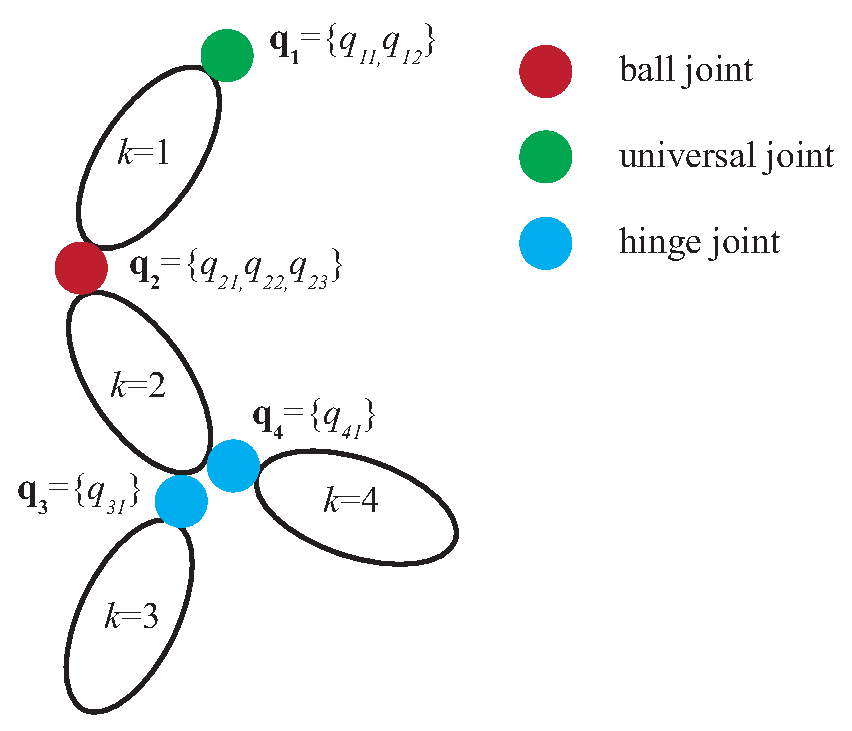
\includegraphics[width=2.1in]{example1_new.eps}
\end{center}
\caption{An articulated system.}
 \vspace{0pt}
\label{fig:example1}
\end{wrapfigure}

We list a few notations and definitions for an articulated rigid body system with $m$ rigid links. 
\begin{itemize}
\item $p(k)$ returns the index of the parent link of link $k$. For
  example in Figure \ref{fig:example1}, $p(4) = 2$. $p(1,k)$ returns the indices of all the links in the chain from the root to the link $k$ (including $k$). For example, $p(1,4) = \{1,2,4\}$
\item $n(k)$ returns the number of DOFs in the joint that connects the  link $k$ to the parent link $p(k)$. For example in Figure \ref{fig:example1}, $n(2) = 3$, $n(3) = 1$ etc. We denote the total number of DOFs in the system by $n$. \eg $n=7$ in Figure \ref{fig:example1}.
\item $R_k$ is the local rotation matrix for the link $k$ and depends only on the DOFs $\vc{q}_k$. $R^0_k$ is the chain of rotational transformations from the
  world frame to the local frame of the link $k$. Therefore, $R^0_k = R^0_{p(k)}R_k$. Since the link $1$ does not have a parent link, $R^0_{p(1)} = \vc{I}_3$.
\end{itemize}



\subsection{Cartesian and generalized velocities}

For a single rigid body, \eqnref{vellin} and \eqnref{velang} describe the relation between the Cartesian velocities and the generalized velocities. 
For an articulated rigid body system, we use the same recipe as rigid body dynamics in \secref{rigidbodydyngen} and define the Jacobians for each rigid link that relate its respective Cartesian velocities to the generalized velocity of the entire system. 

We start with deriving the relation for the angular velocity. The angular velocity of link $k$ viewed in the world frame is:
\begin{eqnarray}
\nonumber
[\bm{\omega}_k] & = & \dot{R}^0_k {R^0_k}^T = \dot{(R^0_{p(k)}R_k)} (R^0_{p(k)}R_k)^T\\
\nonumber
& = & (\dot{R}^0_{p(k)}R_k + {R^0_{p(k)}}\dot{R}_k)  R_k^T {R^0_{p(k)}}^T \\
\label{eq:angvelk_recursive}
& = & \dot{R}^0_{p(k)}{R^0_{p(k)}}^T + R^0_{p(k)} \left ( \dot{R}_k R_k^T \right ) {R^0_{p(k)}}^T \equiv [\bm{\omega}_{p(k)}] + R^0_{p(k)} [\hat{\bm{\omega}}_k] {R^0_{p(k)}}^T
%& = & [\bm{\omega}_{p(k)}] +  [R^0_{p(k)} \hat{\bm{\omega}}_k] = [\bm{\omega}_{p(k)} + R^0_{p(k)} \hat{\bm{\omega}}_k]
\end{eqnarray}
In the above equation, we define [$\hat{\bm{\omega}}_k] = \dot{R_k} R_k^T$ that denotes the angular velocity of the link $k$ in the frame of its parent link $p(k)$ since the rotation matrix $R_k$ is the rotation of the rigid link $k$ with respect to $p(k)$. We can further write $\hat{\bm{\omega}}_k = \hat{J}_{\omega k} \dot{\vc{q}}_k$ where $\hat{J}_{\omega k}$ is the \emph{local} Jacobian matrix that relates the joint velocity of link $k$ to its angular velocity in the frame of the parent link $p(k)$. The dimension of $\hat{J}_{\omega k}$ is $3\times n(k)$. 

Using the property of skew symmetric matrix, $[R \bm{\omega}] = R [\bm{\omega}]
R^T$, we can express \eqnref{angvelk_recursive} in the vector form as:
\begin{eqnarray}
\label{eq:angvelk_iterative}
\nonumber
\bm{\omega}_k & = & \bm{\omega}_{p(k)} + R^0_{p(k)} \hat{J}_{\omega k} \dot{\vc{q}}_k\\
\nonumber
& = & \sum_{l \in p(1,k)} R^0_{p(l)} \hat{J}_{\omega l} \dot{\vc{q}}_l \mbox{\ \ (By unrolling the recursive definition)}\\
& \equiv & J_{\omega k}\dot{\vc{q}}
\end{eqnarray}
where the Jacobian $J_{\omega k}$ is:
\begin{equation}
\label{eq:angular_velocity_jac_link}
J_{\omega k} = \left ( \hat{J}_{\omega 1}\;\; \hdots\;\; R^0_{p(l)} \hat{J}_{\omega l} \;\;\hdots\;\; \vc{0} \;\;\hdots \right )
\end{equation}

Note that the zero matrices \vc{0} of size $3\times n(l)$ in $J_{\omega k}$ correspond to
joint DOFs $\vc{q}_l$ that are \emph{not} in the chain of transformations from the root to the
link $k$. 
Let us look at a couple of examples using the articulated
rigid body system in Figure \ref{fig:example1}:
\begin{eqnarray}
\bm{\omega}_1 &=& (\hat{J}_{\omega 1} \;\; \vc{0}
\;\;\vc{0}\;\;\vc{0}) \dot{\vc{q}}  \nonumber \\
\bm{\omega}_4 &=& (\hat{J}_{\omega 1} \;\; R^0_1\hat{J}_{\omega 2} \;\;
\vc{0} \;\;
R^0_2 \hat{J}_{\omega 4}) \dot{\vc{q}} \nonumber
\end{eqnarray}
where $\hat{J}_{\omega 1} \in \Re^{3\times2}$, $\hat{J}_{\omega 2} \in \Re^{3\times3}$ and $\hat{J}_{\omega 4} \in \Re^{3\times1}$.
Depending on the representation of the rotation $\vc{q}_k$,
$\hat{J}_{\omega k}$ can assume different values and dimensions. For example, if the joint
between link $1$ and link $2$ in Figure \ref{fig:example1} is
represented as three Euler rotations, $R^{(x)}$, $R^{(y)}$, and
$R^{(z)}$ such that $R_2(\vc{q}_2)= R^{(x)}(q_{21}) R^{(y)}(q_{22}) R^{(z)}(q_{23})$, we have:
\begin{equation}
\hat{J}_{\omega 2} = 
\begin{pmatrix}
\begin{array}{c}
1\\
0\\
0
\end{array}
&
R^{(x)} \Bigg (
\begin{array}{c}
0\\
1\\
0
\end{array} 
\Bigg )
&
R^{(x)} R^{(y)}\Bigg (
\begin{array}{c}
0\\
0\\
1
\end{array} 
\Bigg )
\end{pmatrix}
\end{equation}
If the joint is represented as a quaternion or an
exponential map, $\hat{J}_{\omega k}$ does not have a simple form. As an example, the relation between the rotation matrix $R_k$ and the exponential map representation $\vc{q}_k=(q_{k1},q_{k2},q_{k3})$ can be written as:
\begin{equation}
R_k(\vc{q}_k) = e^{[\vc{q}_k]} = \vc{I}_3 + \frac{sin \theta}{\theta} [{\vc{q}}_k] + \frac{1-cos \theta}{\theta^2}[{\vc{q}}_k]^2
\end{equation}
where $\theta = ||\vc{q}_k ||$. The Jacobian $\hat{J}_{\omega k}$ can be derived by equating the result of $\dot{R}_k R_k^T$ to $[\hat{J}_{\omega k} \dot{\vc{q}}_k]$:
\begin{eqnarray}
\nonumber
\hat{J}_{\omega k} & = & R_k \left ( \vc{I}_3 - \frac{1-cos\theta}{\theta^2}[\vc{q}_k] + \frac{\theta - sin \theta}{\theta^3} [\vc{q}_k]^2 \right )\\
 & = & \vc{I}_3 + \frac{1-cos\theta}{\theta^2}[\vc{q}_k] + \frac{\theta - sin \theta}{\theta^3} [\vc{q}_k]^2
\end{eqnarray}
For the case when $\theta \rightarrow 0$, $R_k$ and $\hat{J}_{\omega k}$ can be approximated as follows:
\begin{eqnarray}
R_k & = & \vc{I}_3 + [{\vc{q}}_k] + \frac{1}{2}[{\vc{q}}_k]^2\\
\hat{J}_{\omega k} & = & \vc{I}_3 + \frac{1}{2}[{\vc{q}}_k] + \frac{1}{6}[{\vc{q}}_k]^2
\end{eqnarray}
\ignorethis{
\begin{equation}
\label{eq:angular_velocity_link}
\bm{\omega}_k = (\vc{s}_1 \cdots \vc{s}_{np} \; R^0_{k-1} \vc{t}_1 \cdots
R^0_{k-1} \vc{t}_{nk}\; \vc{0} \cdots \vc{0}) \dot{\vc{q}} = J_{\omega k} \dot{\vc{q}}
\end{equation}
where $np$ is the number of DOFs in the parent chain and $nk$ is the
number of DOFs in the link $k$. 
}
Similar to the angular velocity, the linear velocity of the center of mass of the link $k$
can be expressed in terms of the generalized velocity: 
\begin{equation}
\label{eq:linear_velocity_link}
\vc{v}_k = J_{vk} \dot{\vc{q}}, \;\;\;\mathrm{where}\;\; J_{vk} = \frac{\partial \vc{x}_k}{\partial \vc{q}}=  \frac{\partial W^0_k
  \vc{c}_k}{\partial \vc{q}}.
\end{equation}
where the chain of homogeneous transformations from the world frame to the local
frame of link $k$ is denoted as $W^0_k$. Note that $W^0_k$ is
different from $R^0_k$ in that $W^0_k$ includes the translational
transformations. $\vc{c}_k$ is a constant vector that denotes the center of mass of link $k$ in
its local frame.

We can concatenate the Cartesian velocities into a single vector $\vc{V}_k$ and denote the relation as:
\begin{eqnarray}
\label{eq:vel_relation_link}
\nonumber
\vc{V}_k & = & {J}_k \dot{\vc{q}}\\
\mbox{where } & & 
\vc{V}_k = \left (
\begin{array}{c}
\vc{v}_k\\
\bm{\omega}_k
\end{array}
\right ) \mbox{and\ }
{J}_k = \left (
\begin{array}{c}
J_{vk}\\
J_{\omega k}
\end{array}
\right ) 
\end{eqnarray}


\subsection{Equations of motion}
We now derive the equations of motion of an articulated rigid body system in generalized coordinates. The kinetic energy $T$ of the entire system can be expressed as the sum of kinetic energies of all the rigid links as $T=\sum_k T_k$. Therefore the equations of motion of the system can be computed as:
\begin{eqnarray}
\nonumber
\frac{d}{dt} \left ( \frac{\partial T}{\partial \dot{\vc{q}}} \right ) - \frac{\partial T}{\partial \vc{q}} & = & \frac{d}{dt} \left ( \frac{\partial \sum_k T_k}{\partial \dot{\vc{q}}} \right ) - \frac{\partial \sum_k T_k}{\partial \vc{q}}\\
\nonumber
& = & \sum_k \left ( \frac{d}{dt} \left ( \frac{\partial T_k}{\partial \dot{\vc{q}}} \right ) - \frac{\partial T_k}{\partial \vc{q}} \right )\\
\nonumber
& = & \sum_k \left ( \left( J_k^T M_{ck} J_k \right )\ddot{\vc{q}} + \left( J_k^T M_{ck} \dot{J}_k + J_k^T [\tilde{\bm{\omega}}_k]M_{ck} J_k \right )\dot{\vc{q}} \right )\\
& = &  \sum_k \left( J_k^T M_{ck} J_k \right )\ddot{\vc{q}} + \sum_k\left( J_k^T M_{ck} \dot{J}_k + J_k^T [\tilde{\bm{\omega}}_k]M_{ck} J_k \right )\dot{\vc{q}}
\end{eqnarray}
In deriving the above equation, we use the equations of motion in generalized coordinates for a single rigid body defined in \eqnref{dyngen_vec} subscripted by $k$ for the dynamics of $k^{th}$ link in the multibody system. The Jacobian $J_k$ for the $k^{th}$ link is defined in \eqnref{vel_relation_link}.


\newpage
\section{Conversion between Cartesian and Generalized Coordinates}
In practice, we often want to use third-party rigid body simulators
rather than develop our own. There are a few widely used physics
engines that provide efficient, robust, and fairly accurate rigid body
simulation and collision handling. Open Dynamic Engine (ODE), PhysX, and
Bullet are perhaps the most popular free choices among game developers and
academic researchers. These commercial simulators use the maximal
representation rather than generalized coordinates
described above. That is, these simulators represent each link in the
articulated rigid body system as six DOFs,
leading to a redundant system with additional constraints between
links. A common practice is to develop control algorithms in
generalized coordinates and do forward simulation using a commercial
physics engine, such as ODE. This requires some conversion between
Cartesian and generalized coordinates.

\ignorethis{
\subsection{Definitions}
In the maximal coordinates, the state of an articulated rigid body
system can be expressed as $(\vc{x}_k, R_k, \vc{v}_k,
\boldsymbol{\bm{\omega}}_k)$, where $k = 1, \cdots, m$. Here $\vc{x}_k$ and
$R_k$ are the position and orientation of the rigid link $k$, and $(\vc{v}_k,
\boldsymbol{\bm{\omega}}_k)$ are the linear and angular velocity of the
rigid link $k$ viewed in the world frame. Similarly, we define the
Cartesian force and torque applied on rigid link $k$ as $(\vc{f}_k,
{\bm{\tau}}_k)$, both of which are expressed in the world
frame.
The same articulated rigid body system can be represented in
generalized coordinates. We define the generalized state as $(q_j,
\dot{q}_j)$, where $j = 1, \cdots, n$. The corresponding generalized
forces are then defined as $(Q_1, \cdots, Q_n)$.
}

\subsection{Velocity conversion}

We can concatenate all $2m$ Jacobian matrices corresponding to each link into a single Jacobian
that relates the generalized velocity to the Cartesian velocity of each
link:
\begin{equation}
\vc{V} \equiv 
\left(
\begin{array}{c}
\vc{v}_1 \\
\vdots \\
\vc{v}_m \\
\bm{\omega}_1 \\
\vdots \\
\bm{\omega}_m
\end{array}
\right) = 
\left (
\begin{array}{c}
J_{v1} \\
\vdots \\
J_{vm} \\
J_{\omega 1} \\
\vdots \\
J_{\omega m}
\end{array}
\right) 
\left(
\begin{array}{c}
\dot{\vc{q}}_1\\
\vdots \\
\dot{\vc{q}}_m
\end{array}
\right)  \equiv \left(
\begin{array}{c}
J_v\\
J_{\omega}
\end{array}
\right)\dot{\vc{q}} \equiv J \dot{\vc{q}}
\end{equation}

Typically, the Jacobian $J$ is full column rank because the
number of DOFs in the maximal representation is more than that in the
generalized representation, i.e $6m > n$. To compute $\dot{\vc{q}}$ from $\vc{V}$, we
will end up solving a over-constrained linear system. We can use
pseudo inverse of $J$ to compute $\dot{\vc{q}}$:
\begin{equation}
 \dot{\vc{q}} =  J^+\vc{V}
 \end{equation}
where the pseudo-inverse notation $J^+ = (J^TJ)^{-1}J^T$. If this
least-square solution does not exactly solve the linear
system (i.e. $J \dot{\vc{q}} = \vc{V}$), it indicates that $\vc{V}$ cannot be achieved in the
generalized coordinates without violating constraints of the system
(e.g. constraints that keep links connected).

Computing $J^+$ may be expensive for a system with many rigid links. 
Alternatively, we can rewrite the equation using the relative velocity between a child and a parent link expressed in the local
frame of the parent, instead of using velocities of each link
expressed in the world frame. As an example, we write the simplified expression for the angular velocity of link $k$ using \eqnref{angvelk_iterative} as: 
\begin{eqnarray}
\nonumber
\bm{\omega}_k - \bm{\omega}_{p(k)} & = & R^0_{p(k)}\hat{\bm{\omega}}_k = R^0_{p(k)}\hat{J}_{\omega k} \dot{\vc{q}}_k \\
\Rightarrow \left ( -\vc{I}_3\;\; \vc{I}_3 \right ) 
\left ( 
\begin{array}{c}
\bm{\omega}_{p(k)}\\
\bm{\omega}_k
\end{array}
\right ) & = & R^0_{p(k)}\hat{J}_{\omega k} \dot{\vc{q}}_k
\end{eqnarray}

%\begin{pmatrix}
%\vc{0}  &                    &  &\\
%        & \ddots             &  & \\
%        &                    & R^0_{p(k)}\hat{J}_{\omega k} & \\
%        &                    &  & \ddots & \\
%        &                    &   &     & \vc{0}
%\end{pmatrix} 

Combining these equations for all the links, we get:
\begin{eqnarray}
\label{eq:jacsplit}
\nonumber
D \bm{\omega} = D J_{\omega} \dot{\vc{q}} & = & \mbox{blockdiag}(\hat{J}_{\omega 1},\hdots,R^0_{p(m)}\hat{J}_{\omega m})\dot{\vc{q}}\\
\nonumber
& = & \mbox{blockdiag}(\vc{I}_3,\hdots,R^0_{p(m)})\mbox{blockdiag}(\hat{J}_{\omega 1},\hdots,\hat{J}_{\omega m})\dot{\vc{q}}\\
& \equiv & R \hat{J}_{\omega}\dot{\vc{q}}
\end{eqnarray}
where $D$ is a constant matrix that encodes the connectivity between links. For example, matrix $D$ for the system in Figure \ref{fig:example1} looks
like:
\begin{equation}
D =
\left (
\begin{array}{cccc}
\vc{I}_{3}  & \vc{0} & \vc{0} & \vc{0}\\
-\vc{I}_{3} & \vc{I}_{3}  & \vc{0} & \vc{0}\\
\vc{0} & -\vc{I}_{3} & \vc{I}_{3}  & \vc{0}\\
\vc{0} & -\vc{I}_{3} & \vc{0} & \vc{I}_{3}\\
\end{array}
\right )  
\end{equation}
The relations between $\hat{\bm{\omega}}$ and $\bm{\omega}$, and $\hat{J}_{\omega}$ and $J_{\omega}$ follow from \eqnref{jacsplit}:
\begin{eqnarray}
\label{eq:jacbodyhat}
\nonumber
\hat{\bm{\omega}} & = &R^T D \bm{\omega}\\
\mbox{and } \hat{J}_{\omega} & = & R^T D J_{\omega}
\end{eqnarray}
The matrix $\hat{J}_{\omega}$ being block diagonal is much sparser as compared to ${J}_{\omega}$. 

\ignorethis{
If $\vc{q}$ satisfies the over-constrained system of equations $\vc{V} = J\dot{\vc{q}}$, we need only $n$ constraints out of $6m$ to uniquely determine $\dot{\vc{q}}$ from the Cartesian velocities $\vc{V}$. Equivalently, we can collect $k$ number of rows from $J$ in $J'$ such that the rank of $J'$ is $n$, and compute $\dot{\vc{q}} = J'^+ \vc{V}'$, where $\vc{V}'$ are the velocity components corresponding to the rows in $J'$. This computed $\dot{\vc{q}}$ still satisfies $\vc{V} = J\dot{\vc{q}}$. 
%Therefore, $\dot{\vc{q}}$ computed in \eqnref{angvel_cart2gen} also satisfies the linear velocity relation $\vc{v} = J_v \dot{\vc{q}}$.
}

If $\vc{q}$ satisfies the over-constrained system of equations $\vc{V}
= J\dot{\vc{q}}$, using any $n$ independent constraints out of $6m$ to
solve this linear system will result in the same $\dot{\vc{q}}$. This
can be explained by the problem of fitting an unknown plane to $6m$ 3D
points as $A\vc{x} = \vc{b}$, where $A \in \Re^{6m \times 3}$. If all
$6m$ points happen to lie on a plane, i.e. there exists an $\vc{x}$
that exactly satisfies the over-constrained system, any three
distinctive points we pick as the constraints will result in the same
plane. Therefore, if we know $\vc{V}$ can be achieved in the
generalized coordinates, we can pick a subset of rows from $J$ to form
a $J'$ such that the rank of $J'$ is $n$, and compute $\dot{\vc{q}} =
J'^+ \vc{V}'$, where $\vc{V}'$ are the velocity components
corresponding to the rows in $J'$. The solution $\dot{\vc{q}}$ to this
system will be the same for any $J'$.


For a system with only rotational DOFs, it is sufficient
to invert only $J_{\omega}$ which is also a full column rank matrix
($J_{\omega} \in \Re^{3m \times n}$ and $n\leq 3m$). This is because
each rotational joint can have at most three independent DOFs.  We
then can compute the velocities of the rotational DOFs $\dot{\vc{q}}$
as:
\begin{eqnarray}
\label{eq:angvel_cart2gen}
\nonumber
 \dot{\vc{q}} & = & J_{\omega}^+ \bm{\omega}\\
 \nonumber
 & = &  \hat{J}_{\omega}^+ R^T D\bm{\omega} = \hat{J}_{\omega} \hat{\bm{\omega}} \\
% & = & \mbox{blockdiag}\left(\hat{J}_{\omega 1}^+,\hdots,\hat{J}_{\omega m}^+\right ) \mbox{blockdiag}\left(\vc{I}_3,\hdots,{R^0_{p(m)}}^T\right ) D\bm{\omega}
\nonumber
& = & \mbox{blockdiag}\left(\hat{J}_{\omega 1}^+,\hdots,\hat{J}_{\omega m}^+\right ) \hat{\bm{\omega}}\\
\mbox{or\ \ } \dot{\vc{q}}_k & = & \hat{J}_{\omega k}^+ \hat{\bm{\omega}}_k \mbox{\ \ , } k \in 1\hdots m
\end{eqnarray}
From this formulation, we see that the problem of computing pseudo-inverse of a matrix
$J_{\omega}$ is reduced to computing $m$ pseudo-inverses of much
smaller constant-sized matrices $\hat{J}_{\omega k}$. Note that $\dot{\vc{q}}$ computed in \eqnref{angvel_cart2gen} also satisfies the linear velocity relation $\vc{v} = J_v \dot{\vc{q}}$.

\ignorethis{
Note that if $\vc{V}$ can be achieved in the generalized coordinates,
there exists a unique $\dot{\vc{q}}$ satisfying $\vc{V}' =
J'\dot{\vc{q}}$, where $J'$ is formed by arbitrarily choosing $n$
independent rows from $J$ and $\vc{V}'$ comprises the corresponding
elements in $\vc{V}$. Therefore, if $\vc{V}$ is achievable without
violating the system constraints, $\dot{\vc{q}}$ computed in
\eqnref{angvel_cart2gen} will also satisfy the linear velocity:
$\vc{v} = J_v \dot{\vc{q}}$.}


For systems that include translation DOFs as well, we can separately solve for the rotational DOFs as in \eqnref{angvel_cart2gen} and solve for the translational DOFs for any link $k$ as $\dot{\vc{q}}_k = J_{vk}^+\vc{v}_k$. In most of the cases, only the root joint has translational DOFs making the computation of generalized translational velocities extremely simple as $J_{v1}$ becomes an identity matrix.


\subsection{Force conversion}
The relation between the Cartesian force and the generalized force can
be found in \eqnref{virtual_work}:
\begin{equation}
\label{eq:force_conversion}
\vc{Q} = \sum_k {J^{'}_{vk}}^T \vc{f}_k + J_{\omega k}^T \bm{\tau}^{'}_k = 
\left (
\begin{array}{cc}
{J^{'}_{v}}^T & J_\omega^T
\end{array}
\right)
\left(
\begin{array}{c}
\vc{f} \\
\bm{\tau}^{'}
\end{array}
\right) 
, \;\;\;\mathrm{where}\;\;
J^{'}_{vk} = \frac{\partial \vc{r}_k}{\partial \vc{q}}
\end{equation}
where $\vc{r}_k$ is the point of application of the Cartesian force
$\vc{f}_k$ and $\bm{\tau}^{'}_k$ is the \emph{body torque} applied to link $k$ expressed in the world frame.

\paragraph{Note.} Body torque $\bm{\tau}^{'}_k$ is the torque
applied on link $k$ in the world frame and does \emph{not} include the torque induced by the linear forces $\vc{f}_i$. 
However, the definition for torque in \eqnref{summary_dynamics} \emph{includes} the torque $[\vc{r}_k-\vc{x}_k] \vc{f}_i$ due to each force $\vc{f}_k$ ($\vc{x}_k$ is the COM of the link $i$). As a result, the linear Jacobian $J_{v}$ in \eqnref{summary_dynamics} is defined for the COM of the respective rigid link and $J^{'}_{v}$ in \eqnref{force_conversion} is defined for the point of application of the force. It is easy to verify that ${J^{'}_{vk}}^T\vc{f}_k = J_{vk}^T\vc{f}_k + J_{\omega k}^T[\vc{r}_k-\vc{x}_k] \vc{f}_k$. \ie $\bm{\tau}_k = \bm{\tau}^{'}_k + [\vc{r}_k-\vc{x}_k] \vc{f}_k$.
%However, for the sake of clarity, we use the new definition of the Jacobian in \eqnref{force_conversion} and abuse the notation by denoting it by $J_v$.

Often many controllers (such as a tracking controller) find it convenient to compute the Cartesian-space \emph{joint torques} in the local frame of the parent link rather than body torques in the world frame. Joint torque $\hat{\bm{\tau}}_k$ in the frame of parent link $p(k)$ is defined such that positive torque in the world frame $R^0_{p(k)}\hat{\bm{\tau}}_k$ is applied to the link $k$ and negative torque $-R^0_{p(k)}\hat{\bm{\tau}}_k$ is applied to the parent link $p(k)$. Therefore, the body torque $\bm{\tau}^{'}_k$ applied to the link $k$ can be written in terms of the joint torques as $\bm{\tau}^{'}_k = R^0_{p(k)}\hat{\bm{\tau}}_k - \sum_l R^0_{k} \hat{\bm{\tau}}_l$, $\forall l:k=p(l)$. Collecting the body torques for all the rigid links in the vector $\bm{\tau}$, the relation between the body torques and the joint torques can be defined as:
\begin{eqnarray}
\label{eq:torquesbodyhat}
\bm{\tau}^{'} & = & D^T R \hat{\bm{\tau}} = (R^T D)^T \hat{\bm{\tau}}
\end{eqnarray}
where $R, D$ are defined in \eqnref{jacbodyhat}. We now substitute \eqnref{torquesbodyhat} in \eqnref{force_conversion} and get:
\begin{eqnarray}
\label{eq:torques_cart2gen}
\nonumber
\vc{Q} & = & 
\left (
\begin{array}{cc}
{J^{'}_{v}}^T & J_\omega^T
\end{array}
\right )
\begin{pmatrix}
\vc{f} \\
(R^T D)^T \hat{\bm{\tau}}
\end{pmatrix}
 \\
\nonumber
& = & 
\left (
\begin{array}{cc}
{J^{'}_{v}}^T & (R^T D J_\omega)^T
\end{array}
\right )
\left (
\begin{array}{c}
\vc{f} \\
\hat{\bm{\tau}}
\end{array}
\right )
\\
& = & 
\left (
\begin{array}{cc}
{J^{'}_{v}}^T & \hat{J}_\omega^T
\end{array}
\right )
\left (
\begin{array}{c}
\vc{f} \\
\hat{\bm{\tau}}
\end{array}
\right )  \mbox{\ \ (Using \eqnref{jacbodyhat})}
\end{eqnarray}

\eqnref{torques_cart2gen} gives the relation to convert the given cartesian forces \vc{f} and joint torques $\hat{\bm{\tau}}$ to the generalized forces $\vc{Q}$. 

We now describe the process to convert the given generalized forces $\vc{Q}$ to cartesian forces and torques. In general, the transposed Jacobian in \eqnref{force_conversion} can be inverted using pseudo-inverse to get the Cartesian forces and torques. Note that the relation represents an under-constrained system when solving for $\vc{f}$ and $\bm{\tau}^{'}$. This is because the size of the unknowns is $6m$ and the number of constraints are $n$ with $n\le 6m$. Therefore, we get particular solutions for the Cartesian forces and torques out of many possible solutions.

Based on the information about the form of $\vc{Q}$, we can solve for the Cartesian forces and torques in different ways. We describe the solutions to the following cases:
\begin{enumerate}
\item \textbf{General case. } In the most general case, the points of application of the Cartesian forces are not known. Therefore, we cannot use the Jacobian $J_{v}^{'}$ in \eqnref{force_conversion}. This forces us to assume the points of application to be the COM of each link and compute the torques $\bm{\tau}$ instead of body torques $\bm{\tau}^{'}$. \ie, we can invert the transposed Jacobian by computing its pseudo-inverse and a get a particular least squared solution for $\vc{f}$ and $\bm{\tau}$ as:
\begin{equation}
\left (
\begin{array}{c}
\vc{f} \\
\bm{\tau}
\end{array}
\right ) = \left (
\begin{array}{cc}
{J_{v}}^T & {J}_\omega^T
\end{array}
\right )^+ \vc{Q}
\end{equation}
If the points of the force application are known, the Jacobian in \eqnref{torques_cart2gen} can be inverted to obtain the forces $\vc{f}$ and the joint torques $\hat{\bm{\tau}}$.

\item \textbf{No linear forces. } The more common case for many controllers involves the conversion of only the joint torques from generalized to the Cartesian coordinates. Therefore, the linear forces \vc{f} are zero and \eqnref{torques_cart2gen} can be simplified further to result in the following conversion relation:
\begin{eqnarray}
\nonumber
\hat{\bm{\tau}}  & = & (\hat{J}_{\omega}^T)^+ \vc{Q}\\
\mbox{or } \hat{\bm{\tau}}_k  & = & (\hat{J}_{\omega k}^T)^+ \vc{Q}_k \;\; \forall k \in 1\hdots m
\end{eqnarray}
where $\vc{Q}_k$ denotes the components of the generalized forces corresponding to the rotational DOFs $\vc{q}_k$. Note that the size of the matrix $\hat{J}_{\omega k}^T$ is $n(k)\times 3$ and $n(k)\leq 3$. This implies that we get a particular least squared solution for each $\hat{\bm{\tau}}_k$ out of possibly many solutions that would give rise to the same $\vc{Q}_k$ using the relation $\vc{Q}_k = \hat{J}_{\omega k}^T \hat{\bm{\tau}}_k$.
%\item \textbf{Known points of applied forces. } When the points of application of forces are known, \eqnref{torques_cart2gen} can be used. Instead of inverting the Jacobian,

\end{enumerate}

%\section{Recursive Inverse and Forward Dynamics}


{
%\bibliographystyle{acmsiggraph}
\bibliography{refs}
}

\end{document}
